\documentclass[11pt]{article}

\usepackage[margin=1in]{geometry}
\usepackage{amsmath,amssymb}
\providecommand{\E}{\mathbb{E}}
\usepackage{graphicx}
\usepackage{booktabs}
\usepackage{caption}
\usepackage{hyperref}
\usepackage{natbib}
\usepackage{authblk}
\usepackage{enumitem}

\title{Empirical Analysis of Proposer-Builder Separation on Ethereum: \\
Auction Dynamics, MEV Volatility Clustering, and Market Concentration}

\author[1]{Kyle D. Rothwell\thanks{Stevens Institute of Technology, Department of Computer Science. Email: kdrothwell48@icloud.com.}}
\author[2]{Hao Fu\thanks{Stevens Institute of Technology, Department of Financial Engineering.}}
\affil[1,2]{Working Paper --- Stevens Institute of Technology}

\date{November 2026}

\usepackage{placeins}
\begin{document}

\maketitle

\begin{abstract}
We study Proposer-Builder Separation (PBS) on Ethereum using 1,271,079
delivered payloads from five MEV-Boost relays (September 2024--May 2026) and
every bid recorded for 1,219,842 of those slots in the Relayscan bid archive
\citep{relayscan2024}, 3.7 billion bids in all, the longest-horizon bid-level
study of MEV-Boost auctions to date.

Block values rise with their own recent volatility (Spearman $\rho = 0.494$;
$0.414$ on a non-overlapping earlier window) and with ETH price volatility
($\rho = 0.245$, hourly), but not with the ETH price level ($R^2 = 0.0001$).
Block values are a level process: first-differencing them induces spurious
ARCH effects, so GARCH on ``returns'' is misspecified by construction. On the
AR-filtered level, conditional heteroskedasticity is highly persistent
(GARCH(1,1): $\hat\alpha = 0.044$, $\hat\beta = 0.965$), at the integrated
boundary.

Builders bid under many public keys. Grouping keys by public builder label
and shared blocks, on all 4.1 million MEV-Boost blocks of the period, the HHI
is 344 by key and 3,080 by operator (3,883 with beaverbuild counted in
BuilderNet). It exceeds 2,500 in every week, falls from about 4,600 to 3,500
over the sample, and Titan alone builds 47\% of blocks. Our five-relay sample
under-represents Titan, so auction statistics are re-weighted to market
shares. A median slot receives 2,748 bids from 50 keys and about 25
operators. When the winning bid arrives it stands 1.08\% above the best live
bid of any other operator at the median (zero by key), and the margin narrows
from 2--3\% through mid-2025 to under 0.3\% from late 2025. A rival's live bid is
higher in 18\% of slots, but per-relay traces show such bids are a median of
12\,ms old. Bid timing in the archive's top-bid files differs by over six
seconds across relays, which we trace to the collection channel. Seasonality
by hour and weekday is highly significant.

\vspace{1em}
\noindent\textbf{Keywords:} Proposer-Builder Separation, Maximal Extractable
Value, Ethereum, GARCH, market microstructure, auction theory, decentralised
finance, blockchain economics
\end{abstract}

\newpage
\tableofcontents
\newpage

%==================================================================
\section{Introduction}
\label{sec:intro}
%==================================================================

Ethereum's transition to proof-of-stake consensus, commonly referred to as the
Merge, fundamentally restructured how blocks are produced and how value is
extracted from transaction ordering. Prior to the Merge, miners held full
control over block construction and could exploit that position to extract
Maximal Extractable Value (MEV), which refers to profits arising from the
ability to selectively include, exclude, or reorder transactions within a block
\citep{daian2020}. Following the Merge, Ethereum adopted Proposer-Builder
Separation (PBS) via MEV-Boost \citep{flashbots2022}, separating the roles of
block construction and block proposal into a competitive auction marketplace.
Under PBS, validators (proposers) no longer construct blocks themselves.
Instead, specialized agents called builders assemble blocks designed to maximize
extractable transaction value and submit bids to relay servers. Proposers select
the highest-bidding block header and receive a payment from the winning builder.
This design is intended to democratize MEV by separating it from the staking
process, enabling proposers to capture competitive MEV revenues without
requiring sophisticated order flow infrastructure \citep{buterin2021}.

Despite PBS's importance to Ethereum's economic security and decentralization
goals, several empirical questions remain unresolved. How does MEV opportunity
vary with market volatility conditions? Does block value volatility exhibit the
temporal clustering observed in traditional financial markets? Has builder
competition increased or decreased over time? Are there predictable temporal
patterns in MEV activity? And how competitive is the PBS auction itself---how
many independent operators stand behind the builder keys that bid, how
closely do they compete, and does competition intensify when block values
are highest?

We address these questions using 1,271,079 delivered payload observations from
five MEV-Boost relays spanning September 2024 through May 2026, supplemented by
every bid recorded for 1,219,842 of those slots in the Relayscan.io Bid
Archive \citep{relayscan2024}: 3.7 billion bids from 803 builder keys.
Concentration is measured on the delivered payloads of all relays, 4.1
million blocks \citep{dataalways2024}.
Bid-level studies of MEV-Boost auctions exist \citep{oz2024,wang2024}, but
cover six months or less; the present sample spans 20 months and three market
regimes. To our knowledge, this is the first conditional-heteroskedasticity
analysis of MEV block values; the first to measure concentration and bid
margins by operator, with keys grouped by public label and by shared blocks, over a horizon
of this length; and the first to document that bid timing in the archive's
top-bid files depends on the channel through which each relay's bids were
collected.

The paper is organized as follows. Section~\ref{sec:background} reviews related
work. Section~\ref{sec:data} describes the data. Section~\ref{sec:method}
presents the methodology. Section~\ref{sec:results} reports the findings.
Section~\ref{sec:discussion} discusses implications.
Section~\ref{sec:conclusion} concludes.

%==================================================================
\section{Background and Related Work}
\label{sec:background}
%==================================================================

MEV was first systematically documented by \citet{daian2020}, who identified
transaction-ordering dependencies on Ethereum, documented priority gas auctions
among arbitrage bots, and introduced the notion of miner extractable value. \citet{qin2022} subsequently
conducted a comprehensive empirical assessment across MEV categories, finding
that arbitrage and liquidations account for the majority of extracted value by
magnitude.

PBS was formally proposed by \citet{buterin2021} as a mechanism to decouple MEV
extraction from consensus participation, reducing the centralizing pressure that
MEV imposes on the validator set. The practical implementation, MEV-Boost, was
developed by \citet{flashbots2022} and adopted by the majority of Ethereum
validators following the Merge. \citet{bahrani2024} modelled block building under PBS
and quantified, as a function of the competitiveness of the builder ecosystem,
the extent to which PBS reduces reward heterogeneity across proposers. \citet{wahrstatter2023}
examined builder concentration from a censorship resistance perspective.

The closest antecedents to the auction analysis in this paper are the
bid-level studies of MEV-Boost. \citet{oz2024} analysed six months of bids and
found that builder market share correlates with order-flow diversity while
profitability correlates with exclusive order flow, so that share and margin
are positively correlated among the top builders. \citet{wang2024} documented
that private order flow accounts for roughly 55\% of block value and argued
that this drives the builder market toward monopoly. \citet{wu2023} and
\citet{wu2024} developed game-theoretic models of builder bidding under
latency and showed, by simulation, that a small set of advantaged builders
consolidate the market. The present paper differs in horizon (20 months
against their weeks to six months), in treating the time-series properties of
block values directly, in grouping builder keys into operators before
measuring concentration and margins, and in documenting that bid timing in
the archive's top-bid files depends on the collection channel, which affects
any cross-relay timing analysis in this literature.

Recent empirical work has illuminated the role of CEX-DEX arbitrage in driving
high-value block construction. \citet{heimbach2024} documented a significant
correlation between arbitrage volumes and token price volatility, and showed
that builders integrated with CEX-DEX searchers have greater odds of winning
MEV-Boost auctions during high-volatility periods. \citet{wu2025} estimated that
19 major CEX-DEX searchers extracted \$233.8M USD over a 19-month period, and
demonstrated that exclusive searcher-builder arrangements drive centralization
in both markets. These supply-side findings complement the auction-side evidence
in the present paper: the rise in block values with both block-value and ETH
price volatility documented in Section~\ref{sec:vol_regimes} is consistent with CEX-DEX arbitrage flow as
an important mechanism, while the larger number of operators contesting high-value slots
(Section~\ref{sec:auction}) is consistent with a broader contest when MEV opportunity is elevated.

The volatility modeling in this paper draws on GARCH models as introduced by
\citet{bollerslev1986}, building on \citet{engle1982}'s original ARCH framework.
The Integrated GARCH specification, in which $\alpha + \beta = 1$, was studied
by \citet{engle_bollerslev1986} and is associated with permanent effects of
volatility shocks.

For market structure analysis we use the Herfindahl-Hirschman Index
\citep{hirschman1945}.

%==================================================================
\section{Data}
\label{sec:data}
%==================================================================

\subsection{Delivered Payload Collection}

Data were assembled by querying the public REST APIs of six MEV-Boost relay
operators: Flashbots, Ultra Sound Money, BloXroute (regulated), Aestus,
Agnostic Gnosis, and Eden Network. For each slot, only the highest-value
delivered payload across all relays was retained to avoid double-counting blocks
delivered through multiple relays. Table~\ref{tab:relays} summarizes the records
collected by relay. Eden Network returned no records during the collection
window, so the sample draws on five of the six relays queried.

Relay selection was governed primarily by data availability rather than a
stratified sampling design. These six relays were targeted because they expose
(or were expected to expose) a public, unauthenticated \texttt{delivered\_payloads}
endpoint; relays requiring authenticated access were excluded by necessity.
Within this set, actual coverage varied substantially due to rate limiting,
request timeouts, and differences in API uptime over the collection window, as
reflected in the ``Coverage'' column of Table~\ref{tab:relays}. As a result,
the combined dataset is a convenience sample of publicly-queryable relay data
rather than a representative cross-section of MEV-Boost market share, and is
dominated by BloXroute, which alone contributed approximately 66\% of the
deduplicated sample, and whose records begin only in January 2025; the
September--December 2024 portion of the sample is drawn from Agnostic alone
(Section~\ref{sec:limitations}). The empirical findings in
Section~\ref{sec:results} should
accordingly be understood as characterizing the delivered-payload sequence
observed through this collection process, not the PBS market as a whole;
Section~\ref{sec:limitations} discusses the implications of this composition for
generalizability.

\begin{table}[!htbp]
\centering
\caption{MEV-Boost relay data collection summary}
\label{tab:relays}
\begin{tabular}{lrl}
\toprule
Relay & Records & Coverage \\
\midrule
Flashbots & 58,700 & Partial (rate limited) \\
Ultra Sound Money & 108,000 & Partial (timeout) \\
BloXroute & 1,000,000 & Jan 2025 -- May 2026 \\
Aestus & 16,600 & Partial (timeout) \\
Agnostic & 297,000 & Sep 2024 -- May 2026 \\
Eden Network & --- & Unavailable \\
\midrule
\textbf{Combined (deduplicated)} & \textbf{1,271,079} & \textbf{Sep 2024 -- May 2026} \\
\bottomrule
\end{tabular}
\end{table}

\subsection{Bid Archive Data}

To characterise bidding within the slot, we supplement the delivered payload
dataset with bid-level data from the Relayscan.io Bid Archive
\citep{relayscan2024}, a public archive of MEV-Boost builder bids collected
continuously across all major relays since June 2024. For each calendar day
the archive provides two CSV files: one containing every bid the collector
observed (the ``all-bids'' file, 1.0--2.3\,GB compressed per day in our
period) and one containing top bids only (the ``top-bid'' file, 60--70\,MB).
The auction analysis uses the all-bids files.

Each row of an all-bids file is one bid: the slot, the bid value in Wei, the
hash of the block being offered, the submitting builder's public key, the
relay, and the time at which the relay received the bid relative to slot
start (\texttt{slot\_t\_ms}). Bids reach the archive through three channels:
Ultrasound's top-bid websocket stream, polling of each relay's data API, and
\texttt{getHeader} polling; rows from the last carry no timestamp and are
counted as bids but not used where timing is needed. Bids of $10^{21}$\,Wei
(1{,}000 ETH) or more---almost entirely placeholder bids of approximately
11{,}000 ETH published through \texttt{relay.ethgas.com} from December 2025
onward---were removed, as they are not executable bids.

We read the all-bids file of every day containing a slot of the auction
sample and keep the bids of those slots: 3.70 billion bids over 1,219,842
slots on 598 days. The auction sample is 96.0\% of the 1,271,079 delivered
slots; the remaining 4.0\% fall on 24 days that were not
matched to the archive and are excluded from the auction analysis but
retained in all other analyses. One daily file (12 October 2024) could not be
retrieved. The delivered block of a slot is identified among its bids by
block hash, and is found in 97.9\% of slots (1,193,705). Statistics that need
the arrival time of the winning bid are computed on those slots; counts of
bids, keys and operators use all 1,219,842. Table~\ref{tab:bidarchive}
summarises the dataset.

\begin{table}[!htbp]
\centering
\caption{Bid archive dataset (all-bids files), September 2024 -- May 2026}
\label{tab:bidarchive}
\begin{tabular}{lr}
\toprule
Metric & Value \\
\midrule
Calendar days read & 598 \\
Slots matched to delivered payloads & 1,219,842 \\
Share of delivered slots & 96.0\% \\
Bids in matched slots & 3.70 billion \\
Median bids per slot & 2,748 \\
Median builder keys bidding per slot & 50 \\
Builder keys bidding over the sample & 803 \\
Slots in which the winning block is found among the bids & 97.9\% \\
\bottomrule
\end{tabular}
\end{table}

The much smaller top-bid files are not a substitute, and we state why because
they are the natural first choice. The collector writes a bid to the top-bid
file only if, when it is processed, its value exceeds the highest bid
recorded so far for that slot from any builder, relay or source. Each row is
an improvement to a running maximum, not a builder's best bid, and a bid
that never exceeded the running maximum is not recorded. The record also does
not stop when the auction does: the highest value in a slot's top-bid record
exceeds the delivered (winning) value in 96.2\% of matched slots, by 8.3\% at
the median, and the winning block is itself a row in only 28.8\% of slots.
The median slot has 132 rows from 11 keys in the top-bid file against 2,748
bids from 50 keys in the all-bids file. The top-bid file therefore
identifies neither the winning bid nor the runner-up. We use it only in
Section~\ref{sec:timing_artifact}, where the object of study is the archive
itself.

Two further public datasets are used alongside the archive. Builder labels
come from the Data Always \texttt{mevboost-data} repository
\citep{dataalways2024}, which maps builder public keys to builder names and
records, for every delivered payload on every relay, the builder label
decoded from the block's \texttt{extra\_data} field and the relays that
delivered it. It names the builder for 229 of the 803 keys in our sample;
those keys submit 95.3\% of all bids and win 99.7\% of matched slots. Of the
220 keys that have both a mapped name and an \texttt{extra\_data} label, the
two agree for 218. The same repository's record of delivered payloads covers every relay:
4,105,750 slots in our period, 91.8\% of all slots. Our own sample is 31.0\%
of these; 99.94\% of its slots appear there, each with the same block hash.
We use this complete record, not our sample, to measure concentration
(Section~\ref{sec:concentration}). Per-relay bid traces come from the ethPandaOps Xatu
dataset \citep{xatu2024}, which polls each relay's data API and records
every bid it returns with the relay's name and the relay's own receive
timestamp. Because these files hold 60 to 300 million rows per day, we read
them for a sample of 24 days: the 15th of each month from October 2024 to
April 2026 (16 July in July 2025), 25 November 2025, and 6, 13, 20 and 27 May
2026. They are used only in Section~\ref{sec:same_relay}.

\subsection{Variable Construction}

Block values were converted from Wei to ETH by dividing by $10^{18}$.
Timestamps were derived from slot numbers using the Ethereum Beacon Chain
genesis timestamp $t_0 = 1{,}606{,}824{,}023$ (December 1, 2020) and the fixed
slot duration of 12 seconds:

\begin{equation}
t_{\text{slot}} = t_0 + \text{slot} \times 12
\label{eq:timestamp}
\end{equation}

A common error in Ethereum data analysis is to substitute the Merge timestamp
for genesis, which displaces all computed dates by approximately 21 months (653 days); all
analyses in this paper use the correct genesis timestamp. These slot-derived
timestamps are used directly in Section~\ref{sec:temporal} to assign each delivered payload to
an hour-of-day (UTC) and day-of-week for the temporal pattern analysis.

Log returns were computed as:

\begin{equation}
r_t = \log(1 + v_t) - \log(1 + v_{t-1})
\label{eq:logreturn}
\end{equation}

where $v_t$ denotes block value in ETH at slot $t$. Realized volatility was
estimated using a rolling window of 300 delivered-payload observations:

\begin{equation}
\hat\sigma_t = \sqrt{300} \,\times\, \mathrm{std}(r_{t-299}, \ldots, r_t)
\label{eq:realizedvol}
\end{equation}

Because delivered payloads represent approximately 28\% of all Ethereum slots
over the sample period, consecutive observations in the dataset are not
uniformly spaced in clock time; the 300-observation window covers approximately
3--4 hours of clock time on average rather than one hour.

\subsection{Descriptive Statistics}

The mean block value across the full sample is 0.054 ETH, compared to a median
of 0.016 ETH, with a maximum of 1,243.3 ETH. The large ratio of mean to median
and the extreme upper tail confirm a heavily right-skewed, fat-tailed
distribution in which most blocks carry modest value while rare extreme events
dominate aggregate MEV extraction. These distributional features motivate the
use of non-parametric statistical tests and of Gaussian quasi-maximum
likelihood with robust standard errors in GARCH estimation. All code and data collection scripts are publicly available
at \url{https://github.com/kdrsoccer/pbs-mev-research}; the regime
thresholds, the weekly HHI series and every table in the paper are produced
by the scripts in that repository.

%==================================================================
\section{Methodology}
\label{sec:method}
%==================================================================

\subsection{Volatility Regime Analysis}
\label{sec:method_vol}

Observations were partitioned into three volatility regimes based on the 33rd
and 67th percentiles of the realized volatility series $\hat\sigma_t$
(eq.~\ref{eq:realizedvol}): Low ($\hat\sigma_t \leq 0.6554$), Mid
($0.6554 < \hat\sigma_t \leq 1.4340$), and High ($\hat\sigma_t > 1.4340$),
where 0.6554 and 1.4340 are the empirical 33rd and 67th percentiles of
$\hat\sigma_t$ over the full sample.

Group differences were tested using the Kruskal-Wallis test:

\begin{equation}
H = \frac{12}{n(n+1)} \sum_{i=1}^{k} \frac{R_i^2}{n_i} - 3(n+1)
\label{eq:kruskalwallis}
\end{equation}

where $R_i$ is the rank sum of group $i$ and $n_i$ is the group size. A
directional hypothesis (Low $<$ High) was tested using the Mann-Whitney U test.
The monotone association between realized volatility and block value was measured
by Spearman's $\rho$.

The window in eq.~\ref{eq:realizedvol} ends at, and therefore contains, block
$t$, so an extreme block raises its own measured volatility. We therefore
repeat the comparison with the window ending one block earlier and 300 blocks
earlier (no overlap with block $t$), with block values randomly permuted in
time (a placebo that removes all persistence), and with an external
volatility measure: the 24-hour realized volatility of hourly ETH/USD log
returns, compared with hourly block-value statistics in hours with at least
20 delivered blocks.

The bootstrap procedure used to obtain the confidence interval for
$\hat\rho$ draws $n=8{,}000$ observations via simple random sampling without
replacement from the pooled 1,271,079 observations. Because the underlying
series exhibits volatility persistence (Section~\ref{sec:garch}), this
procedure may understate the true sampling variability of
$\hat\rho$ relative to a block bootstrap that preserves serial dependence; the
reported 95\% CI [0.477, 0.512] should accordingly be treated as a lower bound
on the true confidence interval width.

\subsection{GARCH Volatility Modeling}

Block value is a non-negative level, not a price, and the log return of
eq.~\ref{eq:logreturn} is the first difference of the level series
$u_t = \log(1+v_t)$ (with median $v_t = 0.016$ ETH, $u_t \approx v_t$). First
differencing a level with weak serial dependence produces an MA(1) process
whose squares are positively autocorrelated at lag one and uncorrelated beyond
it, regardless of any volatility dynamics in the level: if $u_t$ were i.i.d.\
with kurtosis $\kappa$, $\operatorname{Corr}(r_t^2, r_{t-1}^2) =
(\kappa-1)/(2\kappa+2)$ exactly. A GARCH model fitted to $r_t$ therefore
responds to this mechanical structure rather than to conditional
heteroskedasticity, and its pseudo-true ARCH coefficient is inflated. We
accordingly model the \emph{level}: $u_t$ is filtered by an AR($p$) regression
($p = 5$ in the main specification; $p = 1$ and $20$ as robustness checks) and
a GARCH(1,1) model is estimated on the residuals $\epsilon_t$ by Gaussian
quasi-maximum likelihood:
\begin{align}
u_t &= c + \sum_{j=1}^{p} \phi_j u_{t-j} + \epsilon_t, \quad \epsilon_t = \sigma_t z_t, \quad \E z_t = 0,\ \E z_t^2 = 1 \label{eq:garchmean} \\
\sigma_t^2 &= \omega + \alpha \epsilon_{t-1}^2 + \beta \sigma_{t-1}^2 \label{eq:garchvar}
\end{align}
Gaussian QMLE is consistent for the conditional-variance parameters under
misspecified innovation distributions \citep{bollerslevwooldridge1992}; a Student-$t$
likelihood with freely estimated degrees of freedom is not used, because on
skewed heavy-tailed differenced levels its unconstrained maximiser has
$\hat\nu$ close to two and $\hat\alpha$ above one, so that a
stationarity-constrained fit returns a boundary solution determined by the
constraint rather than by the data (see Section~\ref{sec:garch}). Volatility persistence
is measured by $\alpha + \beta$; values at or above unity indicate integrated
volatility. We also report, for comparison, the same diagnostics on the
differenced series $r_t$. As delivered payloads are not uniformly spaced in clock time, the
GARCH model characterizes the volatility dynamics of the delivered-payload
sequence rather than a fixed-interval time series.

The recursion in eq.~\ref{eq:garchvar} is itself backward-looking: $\sigma_t^2$
depends only on $\epsilon_{t-1}^2$ and $\sigma_{t-1}^2$, both determined by
information available at or before slot $t-1$. However, the parameters
$\hat\omega, \hat\alpha, \hat\beta$ are estimated via maximum
likelihood over the full 1,271,074-observation sample, so the fitted recursion
at any given slot reflects information from the entire sample period, including
slots occurring later in time. This full-sample estimation is appropriate for
the descriptive characterization of volatility dynamics undertaken here, but
the fitted parameters should not be interpreted as quantities that would have
been observable or usable in real time without re-estimation. Because the
likelihood surface for these series is far from quadratic near the default
starting values used by common software, we estimate by multi-start
derivative-free search (Nelder--Mead from four starting points) followed by
gradient-based polishing.

\subsection{Market Concentration}

Builder identity for each delivered payload is given by the
\texttt{builder\_pubkey} field returned by each relay's
\texttt{delivered\_payloads} endpoint. A public key is not a firm. A single
operator typically bids under many keys, for example one per relay or per
building instance, and concentration measured by key treats each of them as
a separate competitor. We therefore report concentration both by key and by
\emph{operator}.

Operators are defined from two sources. The first is the public label of
each key \citep{dataalways2024}: keys with the same builder label are one
operator. The second is behaviour in the bid archive, which assigns the keys
that have no label: two keys that submit the same block (identical block
hash) are linked, with the strength of a link measured as the number of
shared blocks divided by the number of bids of the less active key on the
days the two are linked, and links weaker than 0.2\% discarded, since two
independent builders can occasionally assemble an identical block. An
operator is a connected component of the graph formed by common labels and
shared-block links. Under this baseline the 803 keys that bid in the sample
form 443 operators, of which 24 hold more than one key and together hold
384 keys.

The 306 keys with a delivered block on any relay belong to 110 operators.

Three alternatives are reported. \emph{Shared blocks only} uses no labels
(497 operators) and shows what the archive alone can recover. \emph{Shared
blocks and value ties} adds a second behavioural link, between two keys
whose highest bids at or below the winning value are equal to the Wei in at
least 200 slots and in at least 2\% of the slots in which the less
frequently present key appears (467 operators). \emph{BuilderNet partners
merged} starts from the baseline and treats beaverbuild, BuilderNet and
Flashbots as one operator (441 operators): beaverbuild and Flashbots operate
BuilderNet \citep{buildernet2024}, and beaverbuild has since retired its own
builder in favour of it \citep{beaverbuild2025}, so their labels do not
identify independent competitors throughout the sample.

Section~\ref{sec:concentration} validates the two behavioural rules against
the labels. In brief, shared blocks never join keys that carry different
labels, while value ties do so once; the baseline therefore does not use
value ties.

The Herfindahl-Hirschman Index was computed weekly:

\begin{equation}
\text{HHI}_w = 10{,}000 \times \sum_i s_{i,w}^2
\label{eq:hhi}
\end{equation}

where $s_{i,w}$ is the share of delivered blocks of key or operator $i$ in
week $w$, so the index lies on the conventional 0--10,000 scale.

Concentration is measured on all MEV-Boost blocks of the period, delivered
through any relay \citep{dataalways2024}, and not on our five-relay sample.
A relay's delivered payloads are not a random draw from the market: builders
differ in which relays they use, so a sample of relays is a sample of
builders. Section~\ref{sec:concentration} shows how far the sample's builder
shares depart from the market's. For the same reason, auction statistics
computed on the sample are also reported re-weighted: each slot is weighted
by the ratio of the market share to the sample share of its winning operator
in its calendar quarter (five largest operators and all others), so that the
weighted sample has the market's composition of winners by quarter.

\subsection{Temporal Pattern Analysis}

Systematic temporal patterns were tested using the Kruskal-Wallis test
(eq.~\ref{eq:kruskalwallis}) separately for hour-of-day (24 groups) and
day-of-week (7 groups), using the slot-derived UTC timestamps from
eq.~\ref{eq:timestamp}.

\subsection{Auction Microstructure Analysis}

For each matched slot $s$ with delivered (winning) value $w_s$, let $o_s$ be
the operator of the winning key and $\tau_s$ the time at which the winning
block was first received by a relay. From all bids of the slot we compute:

\begin{itemize}
\item \textbf{Bids, keys and operators}: the number of bids, the number of
distinct builder keys bidding, and the number of distinct operators bidding.
The per-slot operator count uses shared-block links established within the
same day and no labels, and so slightly overstates the count under the baseline.
\item \textbf{Standing margin}. A builder's new bid replaces its previous
one, so at any moment each key has one live bid, its most recent. Let
$\bar{v}_s$ be the highest live bid, at time $\tau_s$, of any key not
belonging to $o_s$. Then
\begin{equation}
m_s = \frac{w_s - \bar{v}_s}{w_s}
\label{eq:margin}
\end{equation}
is the winner's margin over the best rival operator when the winning bid
arrived. It is negative when a rival's live bid was higher.
\item \textbf{Margin over any lower rival bid}:
\begin{equation}
\ell_s = \frac{w_s - \tilde{v}_s}{w_s}
\label{eq:lead}
\end{equation}
where $\tilde{v}_s$ is the highest bid at or below $w_s$ from any key not
belonging to $o_s$, at any time in the slot. It is non-negative by
construction and includes rival bids that had been replaced, or that arrived
after the winning bid.
\item \textbf{Close rivals}: the number of other operators whose live bid at
$\tau_s$ is at least 99\% of $w_s$.
\item \textbf{Timing}: $\tau_s$, and the time from $\tau_s$ to the next bid
of the winning key.
\end{itemize}

Three features of these measures should be kept in mind. First, the archive
does not record when the proposer requested a header. The request falls
between $\tau_s$ and the next bid of the winning key, which replaces the
winning bid; that interval has a median of 32\,ms, so $\tau_s$ is a close
proxy. Second, the archive stores each bid once, however many relays it was
sent to, so live bids are tracked per key across relays: a key's most recent
bid is treated as its bid on every relay, and timestamps from different
relays are compared directly. A negative $m_s$ can therefore reflect a rival
bid on a relay the proposer did not use, or two bids that arrived within the
resolution of cross-relay timestamps. Section~\ref{sec:same_relay} examines
these slots with per-relay data. Third, both margins depend on which keys
are treated as rivals; we report them under the baseline, the three
alternatives and by key. The margins are computed from the 40 keys with the
highest bids at or below $w_s$ in each slot, of which the eight best rival
groups are retained; 0.11\% of slots have no rival operator among them. We
test associations using Spearman's rank correlation, consistent with the
non-parametric approach used throughout the paper.

\paragraph{Same-relay check.} For the 24 sample days of per-relay traces we
repeat the standing margin on a single relay and a single clock. For each
slot and each relay that both received the winning block and delivered the
payload, let $\tau_{s,r}$ be the time relay $r$ received the winning block.
A rival operator's live bid on $r$ is the most recent bid of any of its
keys received by $r$ no later than $\tau_{s,r}$, and its \emph{age} is
$\tau_{s,r}$ minus the time $r$ received it.

%==================================================================
\section{Empirical Results}
\label{sec:results}
%==================================================================

\subsection{Volatility Regime Effects on Block Values}
\label{sec:vol_regimes}

Table~\ref{tab:regimes} presents distributional statistics for block values
across the three volatility regimes. Mean block value increases monotonically
from 0.0164 ETH in the low-volatility regime to 0.1149 ETH in the
high-volatility regime, a 7.0$\times$ multiple.

\begin{table}[!htbp]
\centering
\caption{Block value (ETH) statistics by volatility regime, September 2024 -- May 2026}
\label{tab:regimes}
\begin{tabular}{lrrrrrr}
\toprule
Regime & Mean & Median & Std Dev & P25 & P75 & P95 \\
\midrule
Low Vol ($n = 419{,}357$) & 0.0164 & 0.0102 & 0.0270 & 0.0070 & 0.0164 & 0.0427 \\
Mid Vol ($n = 432{,}065$) & 0.0313 & 0.0169 & 0.0746 & 0.0107 & 0.0293 & 0.0858 \\
High Vol ($n = 419{,}357$) & 0.1149 & 0.0276 & 2.6463 & 0.0156 & 0.0547 & 0.2136 \\
\bottomrule
\end{tabular}
\end{table}

The Kruskal-Wallis test strongly rejects identical distributions across regimes
($H = 266{,}905.3$, $p < 10^{-300}$, $df = 2$). The Mann-Whitney test confirms
the directional ordering ($p < 10^{-300}$, one-sided). Spearman's rank
correlation is $\rho = 0.494$ ($p < 10^{-300}$, $n = 1{,}270{,}779$).

To confirm stability, we bootstrapped the Spearman correlation across 1,000
random samples of $n = 8{,}000$ observations; the mean bootstrap $\hat\rho =
0.494$ with std.\ dev.\ $= 0.009$ and 95\% CI [0.477, 0.512], confirming the
estimate is stable and not sensitive to any particular subsample.

The 7.0$\times$ multiple, however, is sensitive to how the regimes are
constructed. Because the volatility window contains block $t$, an extreme
block is assigned to the high regime mechanically.
Table~\ref{tab:regime_robust} repeats the comparison with the window shifted
back. The rank correlation is robust (0.490 with the window ending one block
earlier, 0.414 with no overlap), and so is the ratio of medians (2.7, 2.7 and
2.3). The ratio of means is not: it falls to 5.1 and then to 3.5. When block
values are randomly permuted in time, the rank correlation and the ratio of
medians vanish (0.005 and 1.0) but the ratio of means is still 2.5 under the
baseline window, which measures the mechanical component.

\begin{table}[!htbp]
\centering
\caption{Volatility-regime effect under alternative volatility windows.
Ratios compare the high- and low-volatility regimes, defined by the 33rd
and 67th percentiles of each volatility series as in Table~\ref{tab:regimes}.}
\label{tab:regime_robust}
\begin{tabular}{lrrr}
\toprule
Volatility window & Spearman $\rho$ & Ratio of means & Ratio of medians \\
\midrule
Ending at block $t$ (baseline) & 0.494 & 7.0 & 2.7 \\
Ending at block $t-1$ & 0.490 & 5.1 & 2.7 \\
Ending at block $t-300$ (no overlap) & 0.414 & 3.5 & 2.3 \\
Baseline window, values permuted in time & 0.005 & 2.5 & 1.0 \\
\bottomrule
\end{tabular}
\end{table}

An external volatility measure gives the same sign. Across the 14,621 hours
with at least 20 delivered blocks and an ETH price, the hourly median block
value has a rank correlation of 0.245 with the 24-hour realized volatility of
hourly ETH/USD returns and of 0.234 with the absolute hourly return. Mean
block value is 0.035, 0.049 and 0.085 ETH in the low, middle and high
ETH-volatility terciles (2.4$\times$ from low to high); the corresponding
medians of hourly medians are 0.0137, 0.0172 and 0.0210 ETH
(1.5$\times$).

\begin{figure}[!htbp]
\centering
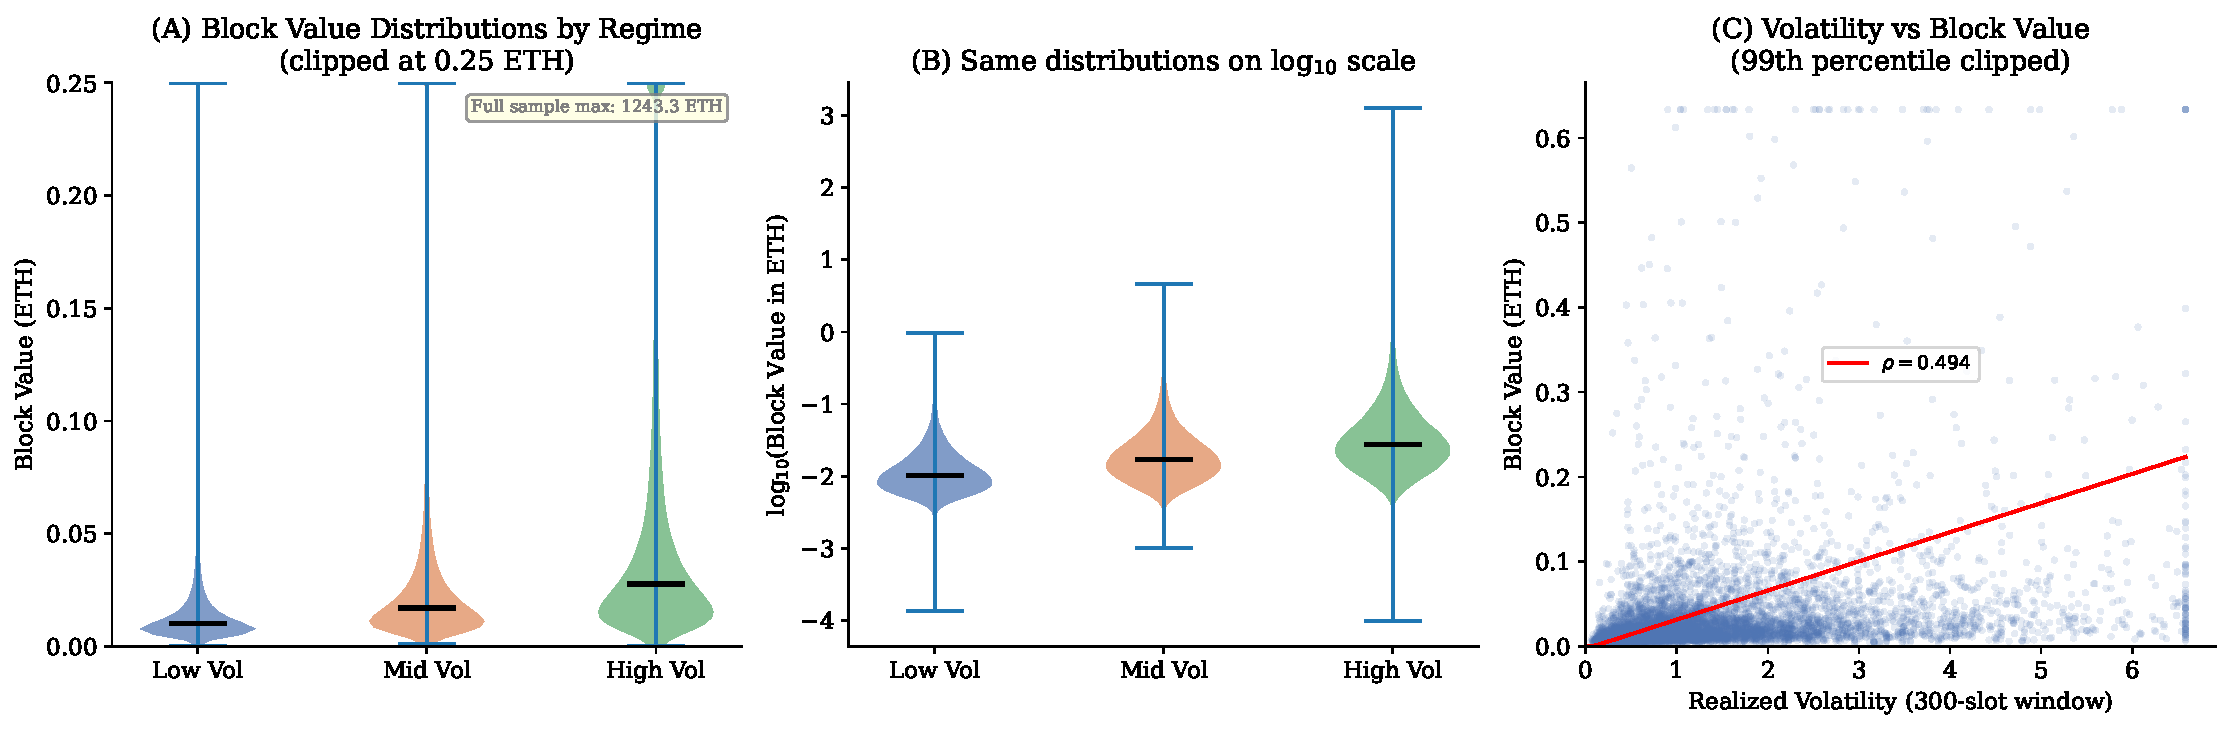
\includegraphics[width=\textwidth]{figures/fig_volatility_regimes.pdf}
\caption{(A) Block value distributions across volatility regimes, clipped at
0.25 ETH for readability. (B) Same distributions on a $\log_{10}$ scale
showing the full range. (C) Scatter of realized volatility against block value
with fitted linear trend. Full-sample Spearman $\rho = 0.494$
($p < 10^{-300}$); bootstrap mean $\hat\rho = 0.494$ (95\% CI: [0.477,
0.512], $B = 1{,}000$ samples).}
\label{fig:regimes}
\end{figure}

\begin{quote}
\textbf{Finding 1.} \textit{Block values are higher when recent volatility
is higher. The rank correlation between block value and realized block-value
volatility is 0.494 ($H = 266{,}905$, $p < 10^{-300}$), and 0.414 when
volatility is measured on a non-overlapping earlier window; the median block
in the high-volatility tercile is 2.3--2.7$\times$ the median in the low
tercile. The ratio of means is 7.0$\times$ under the baseline window but
3.5$\times$ on the non-overlapping window, because extreme blocks raise their
own measured volatility. The association also holds for an external measure:
block values rise with ETH price volatility ($\rho = 0.245$ at hourly
frequency; mean block value 2.4$\times$ higher in the top ETH-volatility
tercile).}
\end{quote}

\subsection{GARCH Dynamics of MEV Block Values}
\label{sec:garch}

Table~\ref{tab:ljungbox} reports Ljung-Box statistics on squared AR(5)
residuals of the level series $u_t$ and, for comparison, on squared
first differences $r_t$. Both reject the no-ARCH null at any conventional level,
but the differenced series does so roughly five times more strongly. The
excess is mechanical: the sample autocorrelation of $r_t$ at lag one is
$-0.425$ (the MA(1) signature of differencing; the i.i.d.-level value is
$-0.5$), and the autocorrelation of $r_t^2$ is $0.434$ at lag one, collapsing
to $0.075$ at lag two. For the level residuals the squared autocorrelations
decay smoothly ($0.135, 0.076, 0.058, 0.047, 0.032$ at lags 1--5), which is the
pattern of genuine volatility persistence.

\begin{table}[!htbp]
\centering
\caption{Ljung-Box tests for ARCH effects}
\label{tab:ljungbox}
\begin{tabular}{lrrr}
\toprule
Series & $Q_{10}$ & $Q_{20}$ & $Q_{50}$ \\
\midrule
Squared AR(5) residuals of level $u_t$ ($n = 1{,}271{,}074$) & 44,779 & 56,366 & 72,464 \\
Squared first differences $r_t$ ($n = 1{,}271{,}078$) & 257,972 & 268,977 & 280,428 \\
\bottomrule
\end{tabular}
\smallskip
\footnotesize All $p < 10^{-300}$. The level residuals have heavy tails, so the statistics should be read as descriptive.
\end{table}

Table~\ref{tab:garch} presents the Gaussian-QMLE GARCH(1,1) estimates on the
AR(5)-filtered level. The ARCH coefficient is small ($\hat\alpha = 0.044$) and
the GARCH coefficient large ($\hat\beta = 0.965$), with
$\hat\alpha + \hat\beta = 1.009$: conditional variance in MEV block values is
highly persistent, at the integrated boundary. Table~\ref{tab:robustness}
shows the estimate is stable across AR filter orders ($p = 1, 5, 20$ give
persistence $1.007$, $1.009$, $1.010$). Across the two halves of the sample
persistence remains near one ($1.002$ and $1.075$), but the parameters do
not: $\hat\alpha$ is $0.044$ in the first half and $0.231$ in the second. The same table reports the fit to the differenced
series: there $\hat\alpha$ rises to $0.539$ and $\hat\beta$ falls to $0.731$,
a twelve-fold inflation of the ARCH term that is the fingerprint of the
differencing artifact described in Section~\ref{sec:method}.

Two cautions. First, $\hat\alpha + \hat\beta \approx 1$ in a 20-month sample
with a known change in relay composition (Section~\ref{sec:limitations}) is
also consistent with shifts in unconditional variance rather than genuine
long-memory volatility \citep{lamoureux1990}; the present analysis does not
distinguish the two. Second, the estimates are sensitive to how the model is
fitted. A Student-$t$ GARCH(1,1) on the differenced series, the
specification that standard practice would suggest, has no interior
solution: its unconstrained maximiser, on differenced heavy-tailed levels,
has $\hat\nu$ close to two and $\hat\alpha$ above one, so a
stationarity-constrained fit returns the boundary
$(\hat\alpha, \hat\beta, \hat\nu) = (0.80, 0.20, 2.7)$, and a single-start
optimiser can return its starting values unchanged. Neither
characterises MEV volatility. Multi-start estimation, Gaussian QMLE, and
modelling the level rather than its difference are each necessary here.

\begin{table}[!htbp]
\centering
\caption{GARCH(1,1) on AR(5) residuals of $\log(1+v_t)$ (residuals scaled by 100), Gaussian QMLE, full 20-month sample}
\label{tab:garch}
\begin{tabular}{lrr}
\toprule
Parameter & Estimate & Robust SE \\
\midrule
$\omega$ (constant) & 0.648 & 0.158 \\
$\alpha$ (ARCH) & 0.044 & 0.010 \\
$\beta$ (GARCH) & 0.965 & 0.007 \\
\bottomrule
\end{tabular}

\smallskip
\footnotesize $\hat\alpha + \hat\beta = 1.009$; log-likelihood $= -4{,}240{,}438$; $n = 1{,}271{,}074$. Residuals in percent of log level (sample variance 85.4). AR(5) coefficients $0.295, 0.124, 0.089, 0.069, 0.072$. Multi-start Nelder--Mead, stationarity constraint not imposed. Standard errors are the robust sandwich form \citep{bollerslevwooldridge1992}, evaluated numerically at the reported estimates; at a near-integrated solution they should be read as approximate.
\end{table}

\begin{table}[!htbp]
\centering
\caption{GARCH(1,1) persistence across specifications (Gaussian QMLE)}
\label{tab:robustness}
\begin{tabular}{llrrr}
\toprule
Series & Sample & $\hat\alpha$ & $\hat\beta$ & $\hat\alpha+\hat\beta$ \\
\midrule
Level, AR(1) residuals & Full & 0.043 & 0.964 & 1.007 \\
Level, AR(5) residuals & Full & 0.044 & 0.965 & 1.009 \\
Level, AR(20) residuals & Full & 0.044 & 0.966 & 1.010 \\
Level, AR(5) residuals & First half & 0.044 & 0.958 & 1.002 \\
Level, AR(5) residuals & Second half & 0.231 & 0.844 & 1.075 \\
\midrule
First differences $r_t$ & Full & 0.539 & 0.731 & 1.270 \\
\bottomrule
\end{tabular}

\smallskip
\footnotesize Stationarity constraint not imposed. The differenced-series row is a diagnostic, not a model of MEV volatility.
\end{table}

\begin{figure}[!htbp]
\centering
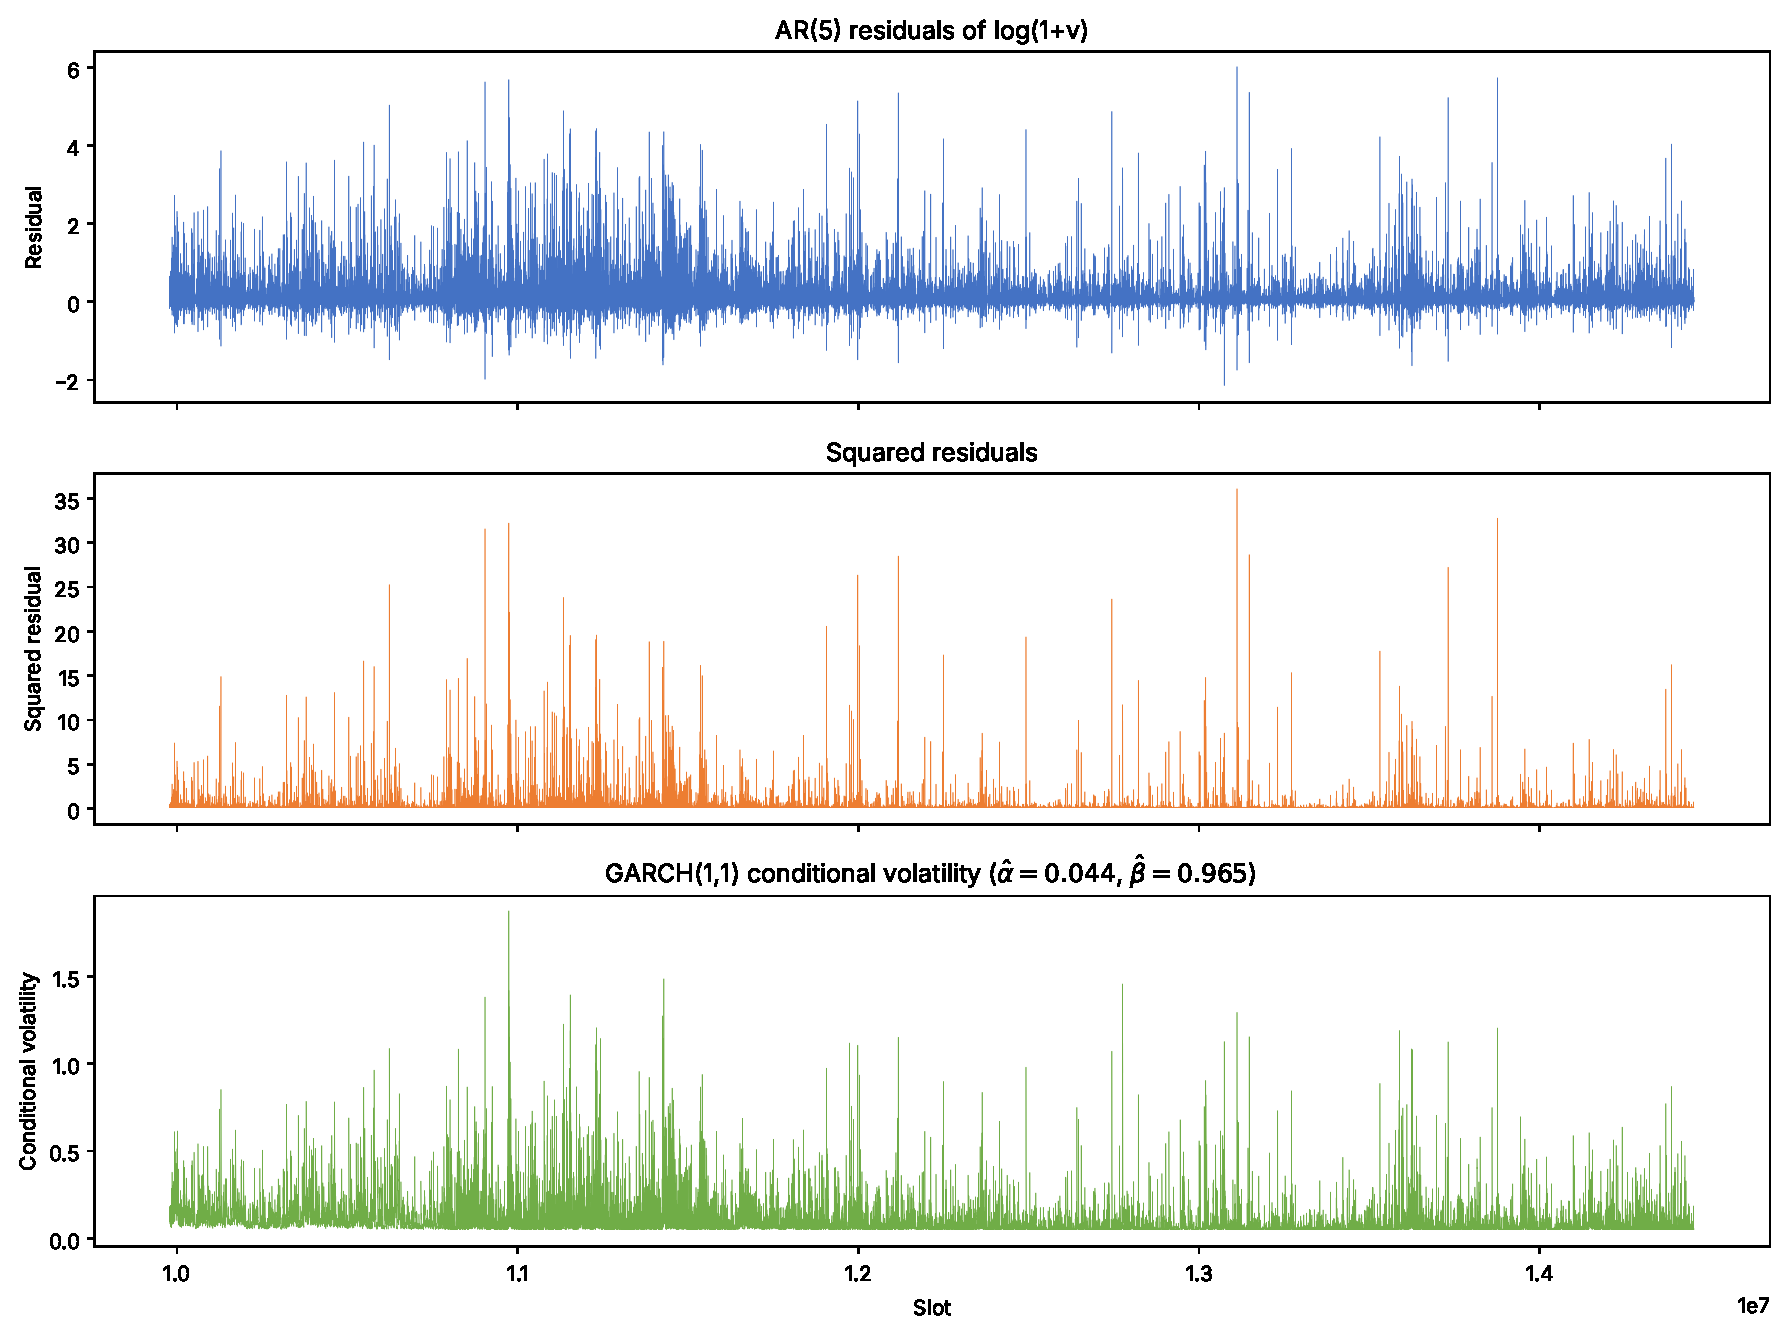
\includegraphics[width=\textwidth]{figures/fig_garch_clustering.pdf}
\caption{Top: AR(5) residuals of $\log(1+v_t)$ across 1,271,074 slots. Middle:
squared residuals. Bottom: GARCH(1,1) conditional volatility
$\hat\sigma_t$ from Table~\ref{tab:garch}.}
\label{fig:garch}
\end{figure}

\begin{quote}
\textbf{Finding 2.} \textit{MEV block values are a level process; first
differencing them manufactures lag-one dependence in squares that mimics ARCH
and makes GARCH on ``returns'' misspecified by construction. Modelled on the
AR-filtered level, block values exhibit highly persistent conditional
heteroskedasticity ($\hat\alpha = 0.044$, $\hat\beta = 0.965$,
$\hat\alpha + \hat\beta = 1.01$), stable across filter orders. Persistence
is near one in both halves of the sample (1.002 and 1.075), though the ARCH
coefficient is larger in the second half. The persistence is at the integrated boundary and may reflect
long-memory volatility or unconditional-variance shifts over the sample.}
\end{quote}

\subsection{Builder Market Concentration}
\label{sec:concentration}

Measured by builder key, block building looks unconcentrated. Across the
4,105,750 MEV-Boost blocks of the period the HHI is 344, the five largest
keys build 30.8\% of blocks, and the weekly HHI lies between 433 and 1,303,
never reaching even the threshold for moderate concentration. Measured by
operator (Section~\ref{sec:method}) it is not. The whole-period HHI is 3,080.
Titan builds 47.0\% of blocks, beaverbuild 21.9\%, BuilderNet 18.1\%, Quasar
7.1\% and rsync 2.6\%: the three largest operators build 87.1\% of blocks
and the five largest 96.8\%. The weekly operator HHI has a median of 3,706,
ranges from 2,879 to 4,746, and exceeds 2,500, the conventional threshold
for a highly concentrated market, in every one of 89 weeks. Key-level
concentration understates operator-level concentration by a factor of nine.

\paragraph{Validation of behavioural linking.} The labels allow the
behavioural rules to be checked (Table~\ref{tab:validation}). Shared blocks
alone never place keys with different labels in one operator, and they put
84\% of labelled bids and 95\% of labelled wins in the largest group of
their label; what they miss is keys of one builder that never submit the
same block, most visibly 17 groups of beaverbuild keys. Adding value ties
recovers more (96\% of bids) at the cost of one false merge: a group of 176
keys that combines Eureka Builder with keys labelled iobuilder, smithbot and
beaverbuild. Two builders that assemble the same transactions would bid the
same value without submitting the same block, so value ties are weaker
evidence of common control than shared blocks, and the baseline does not use
them. Without any labels the market HHI is 2,612 (shared blocks) or 2,910
(with value ties) against 3,080 with them: bidding behaviour alone recovers
85\% to 94\% of the label-based index, against 11\% for keys.

\begin{table}[!htbp]
\centering
\small
\caption{Behavioural linking rules against public builder labels (229
labelled keys)}
\label{tab:validation}
\begin{tabular}{lrrrrr}
\toprule
 & Operators with & Operators with & Purity & \multicolumn{2}{c}{Completeness (\%)} \\
Rule & labelled keys & 2+ labels & (\% of bids) & Bids & Wins \\
\midrule
Shared blocks only & 93 & 0 & 100.0 & 84.2 & 95.2 \\
Shared blocks and value ties & 79 & 1 & 98.0 & 95.7 & 97.2 \\
\bottomrule
\end{tabular}

\vspace{0.5em}
\footnotesize Purity: share of labelled bids in operators' majority label.
Completeness: share of each label's bids (wins) in its largest operator.
The 39 labels would form 39 operators under a perfect rule. Bids and wins
are those of the auction sample.
\end{table}

\paragraph{BuilderNet.} Two of the five largest labels are not independent.
BuilderNet launched in November 2024 operated by Flashbots, beaverbuild and
Nethermind \citep{buildernet2024}, and in May 2025 beaverbuild retired its
own builder to work on BuilderNet \citep{beaverbuild2025}. The handover is
visible in Table~\ref{tab:market}: beaverbuild builds 34.4\% of blocks in
the second quarter of 2025 and 6.6\% in the third, while BuilderNet goes
from 11.4\% to 36.5\%. Treating beaverbuild, BuilderNet and Flashbots as one
operator raises the whole-period HHI to 3,883; the two largest operators
then build 87.2\% of blocks and the three largest 94.3\%. We report both
treatments, since which is appropriate depends on the date and on whether
the question is about infrastructure or about control.

\begin{table}[!htbp]
\centering
\small
\caption{Concentration and builder shares by quarter, all MEV-Boost blocks}
\label{tab:market}
\begin{tabular}{lrrrrrrrrr}
\toprule
 & & \multicolumn{3}{c}{HHI} & \multicolumn{5}{c}{Share of blocks (\%)} \\
Quarter & Blocks & Key & Operator & Merged & Titan & BuilderNet & beaverbuild & Quasar & rsync \\
\midrule
2024 Q3 & 88{,}706 & 771 & 4{,}627 & 4{,}761 & 45.3 & 0.0 & 50.6 & 0.0 & 1.8 \\
2024 Q4 & 602{,}897 & 758 & 4{,}594 & 4{,}711 & 43.2 & 0.5 & 52.1 & 0.0 & 2.6 \\
2025 Q1 & 585{,}776 & 708 & 3{,}989 & 4{,}126 & 43.1 & 1.5 & 45.4 & 0.0 & 8.4 \\
2025 Q2 & 600{,}380 & 573 & 3{,}258 & 4{,}043 & 43.8 & 11.4 & 34.4 & 3.9 & 3.7 \\
2025 Q3 & 611{,}179 & 407 & 3{,}737 & 4{,}218 & 48.2 & 36.5 & 6.6 & 5.4 & 1.0 \\
2025 Q4 & 606{,}439 & 587 & 3{,}525 & 3{,}671 & 49.8 & 29.4 & 2.5 & 12.7 & 2.2 \\
2026 Q1 & 601{,}035 & 675 & 3{,}617 & 3{,}667 & 51.0 & 27.9 & 0.9 & 15.4 & 0.0 \\
2026 Q2 & 409{,}338 & 707 & 3{,}510 & 3{,}580 & 51.9 & 23.2 & 1.5 & 16.3 & 0.0 \\
\bottomrule
\end{tabular}

\vspace{0.5em}
\footnotesize Operator: labels and shared blocks. Merged: beaverbuild,
BuilderNet and Flashbots as one operator. The first and last quarters are
partial (from 17 September 2024; to 31 May 2026).
\end{table}

Concentration is lower at the end of the sample than at the start, and
still high. The operator HHI is about 4,600 in late 2024, when Titan and
beaverbuild together build over 95\% of blocks, and between 3,500 and 3,750 from
the third quarter of 2025. Titan's share does not fall; it rises from 43\%
to 52\%. The decline comes from the other side of the former duopoly: the
beaverbuild and BuilderNet labels together go from 52\% of blocks in late
2024 to 25\% in the last quarter, and most of the difference goes to
Quasar, which builds its first block in April 2025 and 16\% of blocks a year
later. With the BuilderNet partners merged the index falls from about 4,750
to 3,600. rsync disappears from the market in 2026.

\paragraph{The five-relay sample.} Our own delivered-payload sample gives a
different and misleading picture (Figure~\ref{fig:market}). Over the whole
period it puts Titan at 35.4\% of blocks against 47.0\% in the market, and
Quasar at 13.7\% against 7.1\%; its operator HHI is 2,341 against 3,080. By
quarter the gaps are larger: in late 2024, when the sample is drawn from
one relay, Titan has 85\% of sample blocks and 43--45\% of the market, and
in the first quarter of 2026 it has 20\% of sample blocks and 51\% of the
market. A study using this sample alone would conclude that Titan's share
fell by half over a period in which it rose. The cause is that builders
deliver through different relays, and the sample has no blocks from Titan's
own relay and few from Ultra Sound. Any concentration figure computed from a
subset of relays inherits this problem.

\begin{figure}[!htbp]
\centering
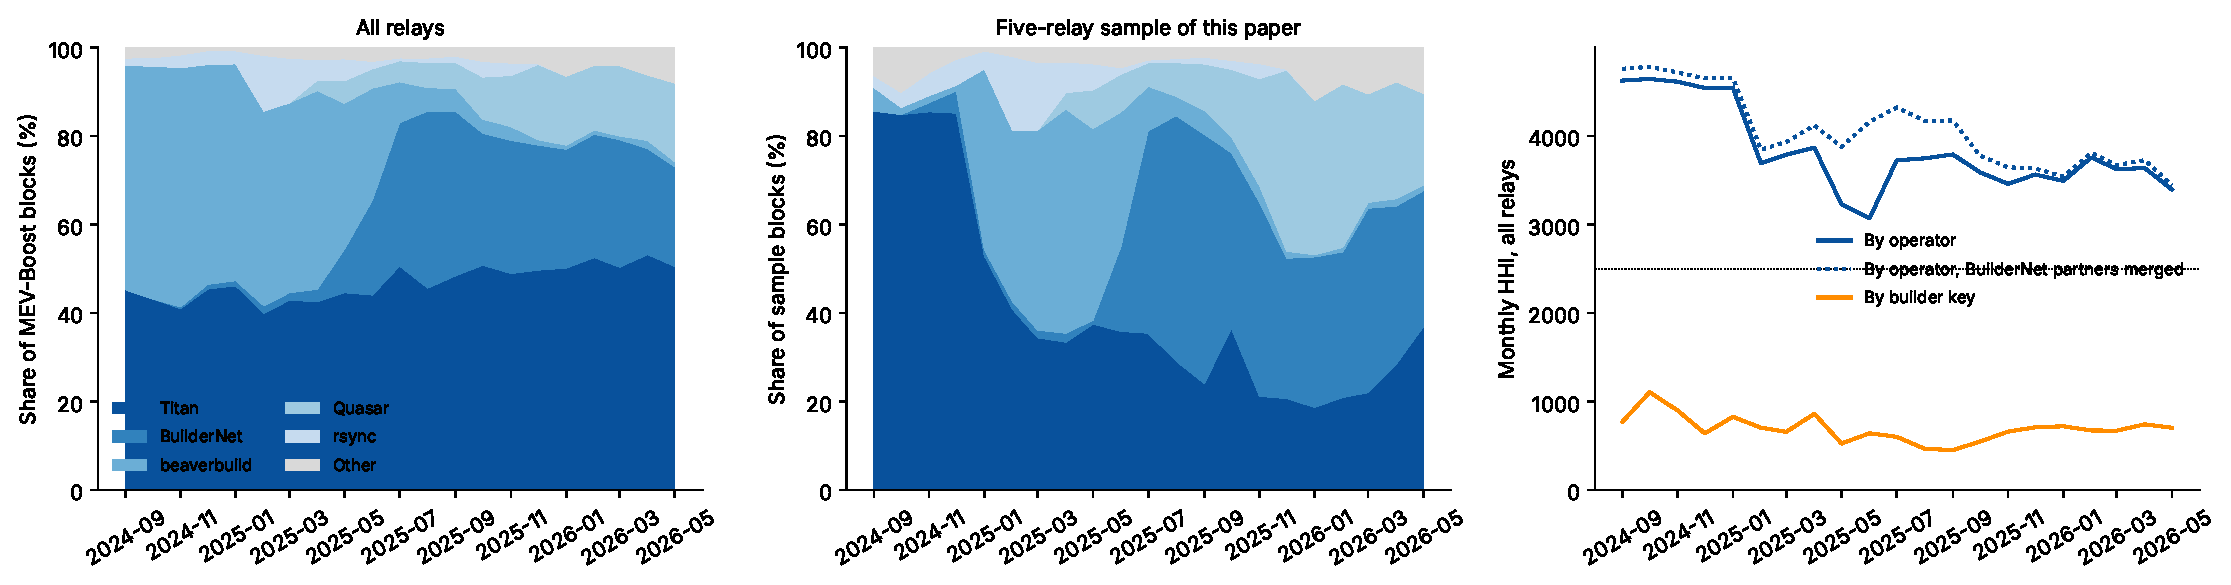
\includegraphics[width=\textwidth]{figures/fig_market_operators.pdf}
\caption{Left: monthly share of all MEV-Boost blocks by operator. Centre:
the same shares in the five-relay sample of this paper. Right: monthly HHI
of all MEV-Boost blocks by operator, by operator with the BuilderNet
partners merged, and by builder key; the dotted horizontal line marks
2,500.}
\label{fig:market}
\end{figure}

\begin{quote}
\textbf{Finding 3.} \textit{Block building is highly concentrated once
builder keys are grouped into operators. Across all 4.1 million MEV-Boost
blocks the HHI is 344 by key and 3,080 by operator (2,612 from bidding
behaviour alone, 3,883 with beaverbuild counted as part of BuilderNet);
Titan builds 47\% of blocks and five operators 97\%, and the weekly operator
HHI exceeds 2,500 in every week. The index falls from about 4,600 in late
2024 to about 3,500, as Quasar enters and the beaverbuild and BuilderNet
share halves, while Titan's share rises from 43\% to 52\%. A sample of five
relays mis-states these shares badly: it shows Titan at 20\% in a quarter
when it built 51\%.}
\end{quote}

\subsection{Temporal Patterns in MEV Activity}
\label{sec:temporal}

Figure~\ref{fig:temporal} displays mean block values by hour of day (UTC) and
day of week. The Kruskal-Wallis test rejects equal distributions across hours
($H = 65{,}875$, $df = 23$, $p < 10^{-300}$) and across days of the week
($H = 33{,}590$, $df = 6$, $p < 10^{-300}$). Block values are highest on
Monday (mean 0.086 ETH) and lowest on Saturday (0.031 ETH). The intraday
pattern is clearest in medians: median block value rises from approximately
0.012--0.013 ETH during 03:00--05:00 UTC to 0.020--0.024 ETH during
13:00--17:00 UTC, consistent with elevated activity during US trading hours.
Hourly means are dominated by a small number of extreme blocks (the 02:00 UTC
mean, for example, reflects a single outlier with hourly standard deviation
5.5 ETH) and should be read with that caveat.

\begin{figure}[!htbp]
\centering
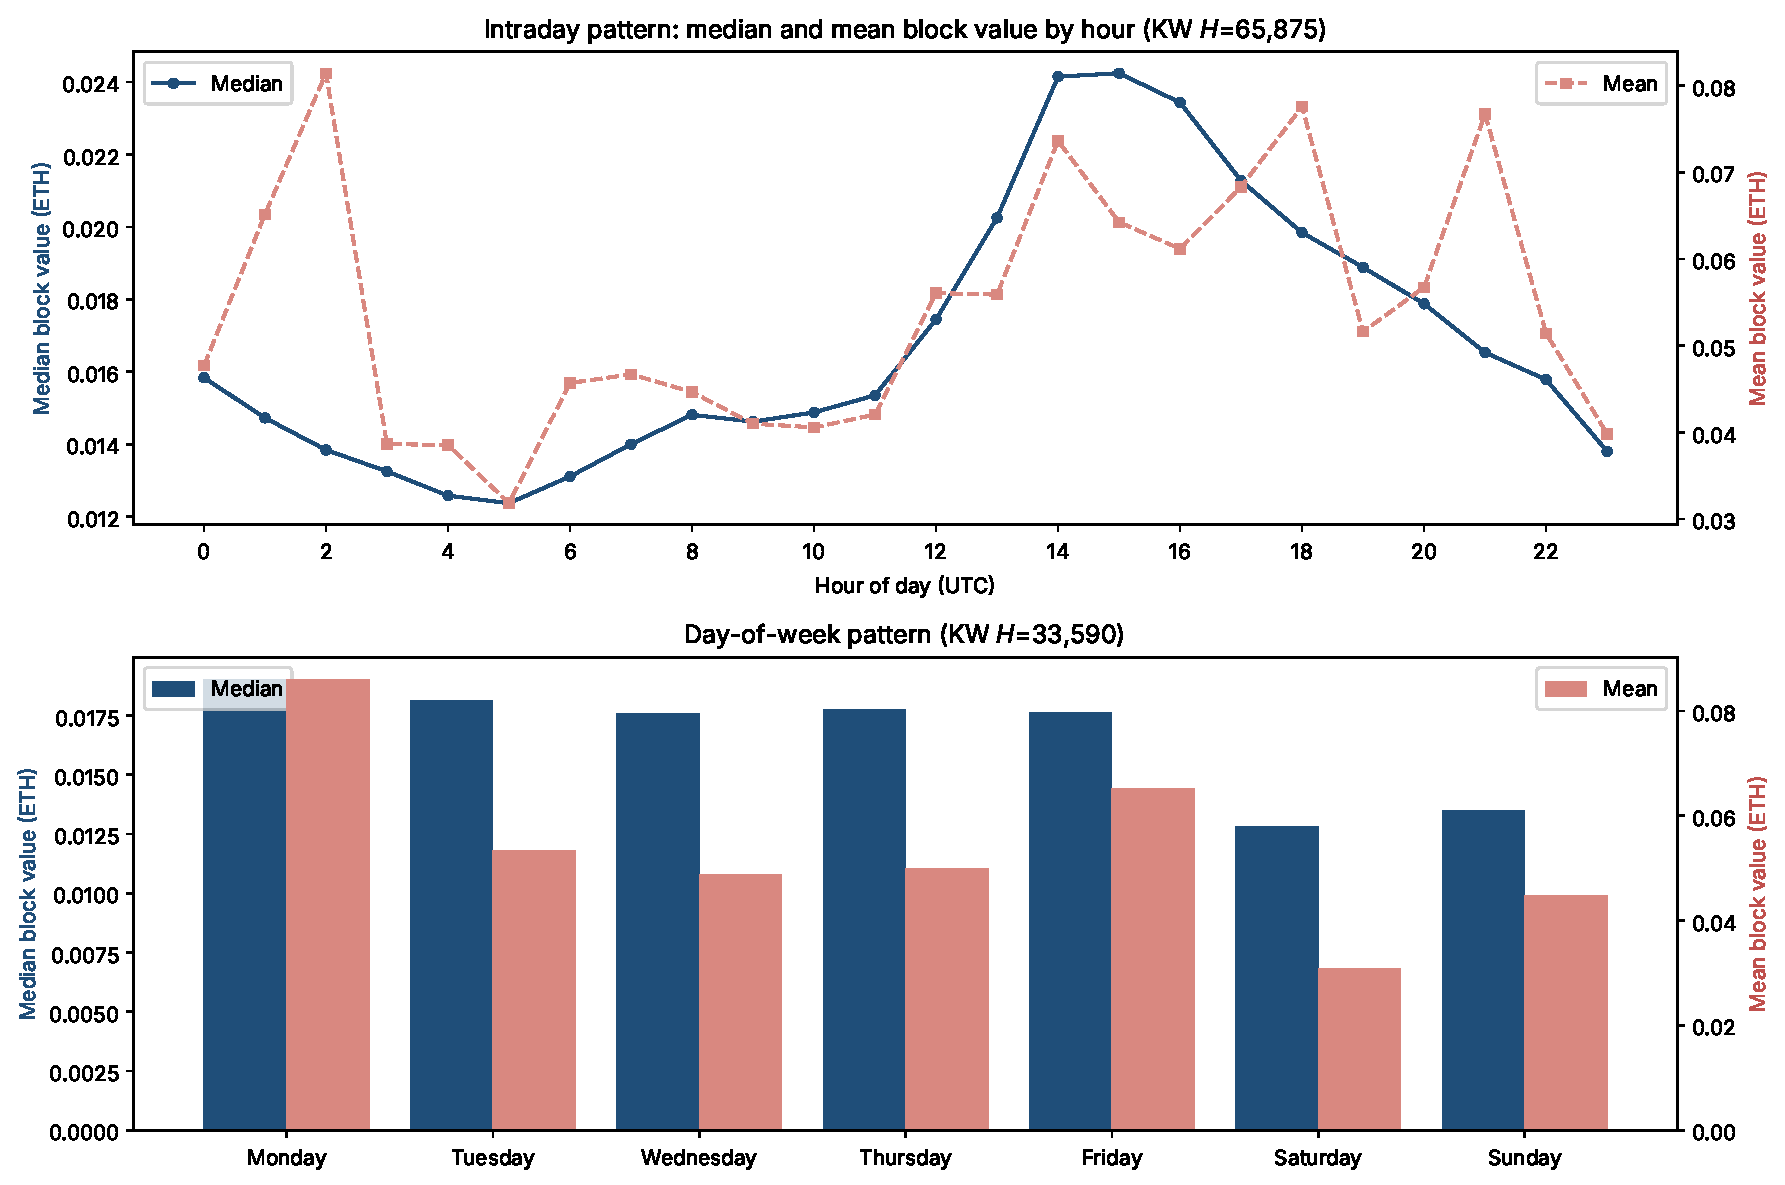
\includegraphics[width=\textwidth]{figures/fig_temporal_patterns.pdf}
\caption{Top: Mean block value by hour of day (UTC); isolated spikes reflect
individual extreme blocks rather than systematic patterns. Bottom: Mean block
value by day of week. Both panels show statistically significant variation
($p < 10^{-300}$).}
\label{fig:temporal}
\end{figure}

\begin{quote}
\textbf{Finding 4.} \textit{MEV block values exhibit statistically significant
intraday and day-of-week seasonality ($p < 10^{-300}$ in both cases). Median
block values peak during 13:00--17:00 UTC and are highest on Monday and
lowest on Saturday.}
\end{quote}

\subsection{Auction Microstructure}
\label{sec:auction}

\subsubsection{Bids, Operators and Margins}
\label{sec:overall_comp}

Table~\ref{tab:auction_summary} presents summary statistics across the
1,219,842 matched slots. The median slot receives 2,748 bids from 50 builder
keys, behind which stand about 25 operators. The winning bid arrives a
median of 968\,ms after slot start (10th percentile 517\,ms, 90th percentile
2,069\,ms; 3.0\% arrive before slot start), and the winning key bids again a
median of 32\,ms later.

\begin{table}[!htbp]
\centering
\caption{Auction summary statistics from all recorded bids ($n = 1{,}219{,}842$ matched slots)}
\label{tab:auction_summary}
\begin{tabular}{lrrrr}
\toprule
Metric & Mean & Median & P10 & P90 \\
\midrule
Bids per slot & 3{,}033 & 2{,}748 & 1{,}361 & 5{,}094 \\
Builder keys bidding & 51.8 & 50 & 39 & 68 \\
Operators bidding & 25.4 & 25 & 20 & 33 \\
Standing margin $m_s$ (\%) & 1.515 & 1.333 & $-$1.265 & 8.367 \\
Margin over any lower rival bid $\ell_s$ (\%) & 1.411 & 0.200 & 0.008 & 3.436 \\
Winning bid arrival $\tau_s$ (ms) & 1{,}100 & 968 & 517 & 2{,}069 \\
Time to the winning key's next bid (ms) & 92 & 32 & 4 & 238 \\
\bottomrule
\end{tabular}

\vspace{0.5em}
\footnotesize Margins and timing are computed on the 1,193,705 slots in
which the winning block is found among the bids, under the baseline operator
definition.
\end{table}

When the winning bid arrives, it stands 1.33\% above the best live bid of
any other operator at the median. The distribution is wide
(Figure~\ref{fig:auction_competitiveness}): the interquartile range is
0.07\% to 4.33\%, the winner is more than 1\% ahead of every rival in
54.7\% of slots and more than 5\% ahead in 20.6\%. Counting rivals instead of
measuring the gap gives the same picture: no other operator has a live bid
within 1\% of the winning bid in 54.8\% of slots, exactly one does in
37.1\%, and two or more do in 8.1\%.

These are statistics of the sample's slots, and the sample has too few
Titan-won slots (Section~\ref{sec:concentration}). That matters, because the
margin depends strongly on who wins (Table~\ref{tab:winner}). When Titan
wins, the median margin is 0.33\% and no rival is within 1\% in a third of
slots; when beaverbuild wins, the median margin is 3.98\% and no rival is
within 1\% in 82\% of slots. Re-weighting the sample to the market's
composition of winners by quarter (Section~\ref{sec:method}) lowers the
median standing margin from 1.33\% to 1.08\%, and the share of slots with no
rival within 1\% from 54.8\% to 51.1\%. We treat the re-weighted figures as
the estimates for the market.

\begin{table}[!htbp]
\centering
\caption{The standing margin by winning operator}
\label{tab:winner}
\begin{tabular}{lrrrrr}
\toprule
 & \multicolumn{2}{c}{Share of slots (\%)} & Median & Rival bid & No rival \\
Winner & Sample & Market & $m_s$ (\%) & higher (\%) & within 1\% (\%) \\
\midrule
Titan & 34.5 & 47.0 & 0.33 & 19.7 & 33.3 \\
BuilderNet & 23.3 & 18.1 & 1.27 & 29.5 & 53.2 \\
beaverbuild & 18.8 & 21.9 & 3.98 & 7.6 & 82.1 \\
Quasar & 13.8 & 7.1 & 2.09 & 11.8 & 70.5 \\
rsync & 4.3 & 2.6 & 1.46 & 19.2 & 57.0 \\
All others & 5.2 & 3.2 & 1.74 & 18.3 & 62.1 \\
\midrule
Sample & & & 1.33 & 18.5 & 54.8 \\
Re-weighted to market & & & 1.08 & 17.6 & 51.1 \\
\bottomrule
\end{tabular}
\end{table}

The second margin bounds the contest from the other side. At some point in
the slot, a rival operator bid within 0.20\% of the winning value at the
median, and within 1\% in 75.0\% of slots. Rivals do reach the neighbourhood
of the winning bid in most slots; what the standing margin adds is that in
more than half of slots none of them is there when the winning bid lands.

\begin{table}[!htbp]
\centering
\small
\caption{Concentration and margins by operator definition}
\label{tab:linking}
\begin{tabular}{lrrrrr}
\toprule
 & Operators & HHI, all & Median & Median & Rival bid \\
Rivals defined by & bidding & MEV-Boost blocks & $m_s$ (\%) & $\ell_s$ (\%) & higher (\%) \\
\midrule
Builder key & 803 & 344 & 0.000 & 0.000 & 36.5 \\
Shared blocks only & 497 & 2{,}612 & 0.737 & 0.117 & 21.1 \\
Shared blocks and value ties & 467 & 2{,}910 & 0.908 & 0.149 & 20.0 \\
Labels and shared blocks (baseline) & 443 & 3{,}080 & 1.333 & 0.200 & 18.5 \\
BuilderNet partners merged & 441 & 3{,}883 & 1.494 & 0.227 & 17.8 \\
\bottomrule
\end{tabular}

\vspace{0.5em}
\footnotesize Margins are those of the sample, not re-weighted.
\end{table}

Table~\ref{tab:linking} shows how much these numbers depend on who is counted
as a rival. By key, both margins are zero at the median: the closest
``competitor'' to the winning bid is typically another key of the same
operator bidding the same value, which is why keys must be grouped before a
margin means anything. Each step towards a more complete grouping widens the
margin, from 0.74\% with shared blocks alone to 1.33\% with labels and
1.49\% with the BuilderNet partners merged, because each removes sibling
keys that were being counted as rivals. The label-based figures are the ones
we rely on; the behavioural ones show the direction of the error when labels
are not available.

\begin{figure}[!htbp]
\centering
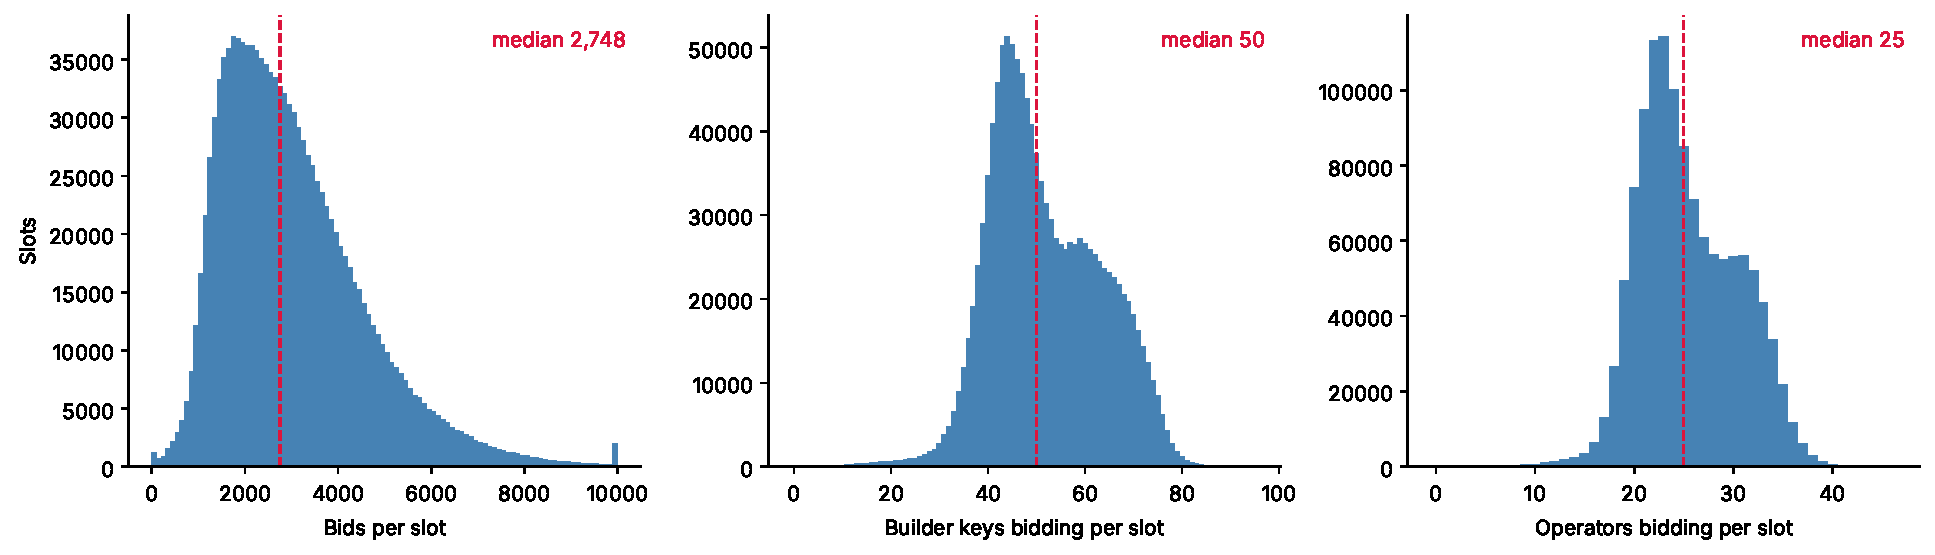
\includegraphics[width=\textwidth]{figures/fig_ab_overview.pdf}
\caption{All recorded bids, 1,219,842 matched slots. Left: bids per slot,
clipped at 10,000 (median 2,748). Centre: builder keys bidding (median 50).
Right: operators bidding (median 25).}
\label{fig:auction_overview}
\end{figure}

\begin{figure}[!htbp]
\centering
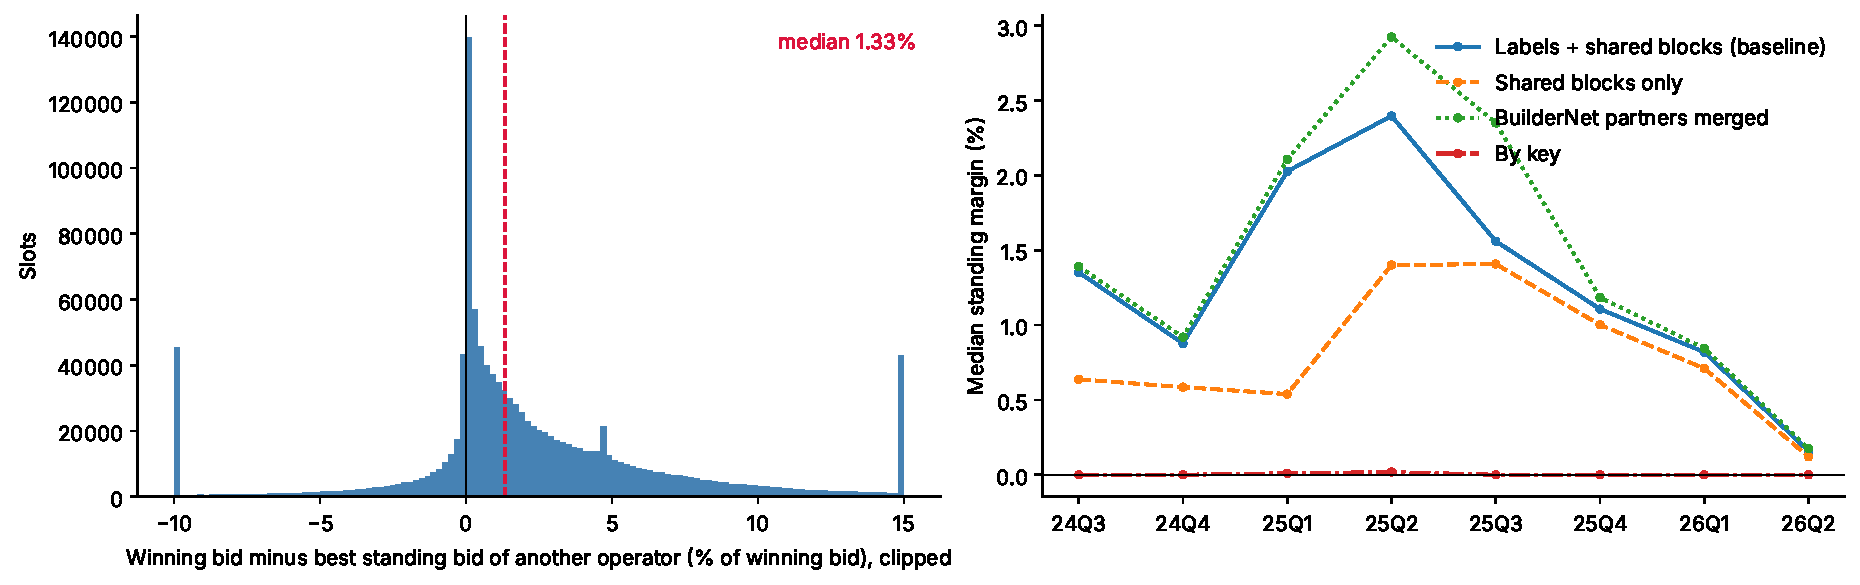
\includegraphics[width=\textwidth]{figures/fig_ab_margin.pdf}
\caption{Standing margin $m_s$: the winning bid minus the best live bid of
another operator when the winning bid arrived, as a share of the winning
bid. Left: distribution, clipped at $-10\%$ and $15\%$ (median 1.33\%).
Right: median by quarter under the baseline, two alternatives and by key.}
\label{fig:auction_competitiveness}
\end{figure}

\subsubsection{When a Rival's Live Bid Is Higher}
\label{sec:same_relay}

The standing margin is negative in 18.5\% of slots, and below $-1\%$ in
10.8\%: according to the archive, a rival operator's live bid was above the
bid the proposer took. Read literally this would mean proposers forgo value
in nearly one slot in five. The archive cannot test that reading, because it
stores each bid once and so cannot say whether the rival's bid was on the
relay the proposer used. The per-relay traces can
(Section~\ref{sec:method}).

The check covers 48,787 slots on the 24 sample days, in which the archive
measure is negative in 20.0\% of slots. On a relay that delivered the block,
measured on that relay's own clock, a rival operator has a higher live bid
in 14.0\% of slots. These bids are very recent. The higher rival bid reached
the relay a median of 12\,ms before the winning block did (interquartile
range 4 to 42\,ms); 77\% are less than 50\,ms old and 83\% less than
100\,ms. A rival bid that was higher and had been on the delivering relay
for at least 100\,ms is present in 2.4\% of slots
(Figure~\ref{fig:relay_trace}).

Of the slots the archive marks as negative, the higher rival bid is found on
a delivering relay in 49.1\%, on another relay only in 18.4\%, and on no
relay covered by the traces in 32.5\%. Coverage limits the last two figures:
the traces contain no Ultra Sound bids after April 2025 and include the
winning block in only 19\% of slots on Titan Relay, so a bid ``not found''
may have been on either.

The picture is therefore of a race in time, not of forgone value. A relay
timestamps a bid when it is received, and two bids received within a few
milliseconds of each other cannot be ordered by receive time alone, still
less across relays. The share of slots with a higher rival bid rises sharply
in the last quarter of the sample, to 37.0\% in the archive and 27.1\% on
the delivering relay, but the share with one at least 100\,ms old is 2.4\%
there too (Table~\ref{tab:same_relay}): rivals are arriving closer together
in time, not being passed over.

The bids that are both higher and at least 100\,ms old are mostly not from
the main competitors. bobthebuilder holds 38\% of them and bloXroute's own
builder 18\%, and the median such bid is 33\% above the winning bid, which
is not a price a competitive builder leaves standing for most of a second;
these look like bids the proposer could not select. One day, 15 December
2024, accounts for much of the fourth-quarter 2024 figure: on BloXroute that
day 27\% of slot-relay pairs have one, and without that day the overall
share is 2.1\%. The five largest operators hold 19\% of the old higher bids,
with a median excess of 1.6\%, and a slot has one from any of them in 0.55\%
of cases. That, not 18.5\%, is the order of magnitude of slots in which a
proposer took a bid while a main competitor's better bid had been visibly
available on the same relay. On the same slots the median margin on the
delivering relay is 1.40\%, against 1.09\% for the archive measure, and the
two are correlated at $\rho = 0.67$.

\begin{table}[!htbp]
\centering
\caption{Slots with a rival live bid above the winning bid: bid archive
against the delivering relay (24 sample days)}
\label{tab:same_relay}
\begin{tabular}{lrrrr}
\toprule
 & & Bid archive, & \multicolumn{2}{c}{On a delivering relay (\%)} \\
Quarter & Slots & across relays (\%) & Any age & At least 100\,ms old \\
\midrule
2024 Q4 & 2{,}031 & 13.0 & 25.1 & 12.1 \\
2025 Q1 & 10{,}979 & 12.0 & 10.1 & 3.0 \\
2025 Q2 & 6{,}542 & 10.5 & 5.9 & 1.5 \\
2025 Q3 & 5{,}602 & 14.0 & 11.1 & 0.8 \\
2025 Q4 & 7{,}270 & 19.5 & 11.7 & 1.4 \\
2026 Q1 & 5{,}758 & 23.7 & 8.6 & 2.1 \\
2026 Q2 & 10{,}605 & 37.0 & 27.1 & 2.4 \\
\midrule
All & 48{,}787 & 20.0 & 14.0 & 2.4 \\
\bottomrule
\end{tabular}

\vspace{0.5em}
\footnotesize The fourth quarter of 2024 is three days; 15 December 2024 on
BloXroute accounts for most of its last column.
\end{table}

\begin{figure}[!htbp]
\centering
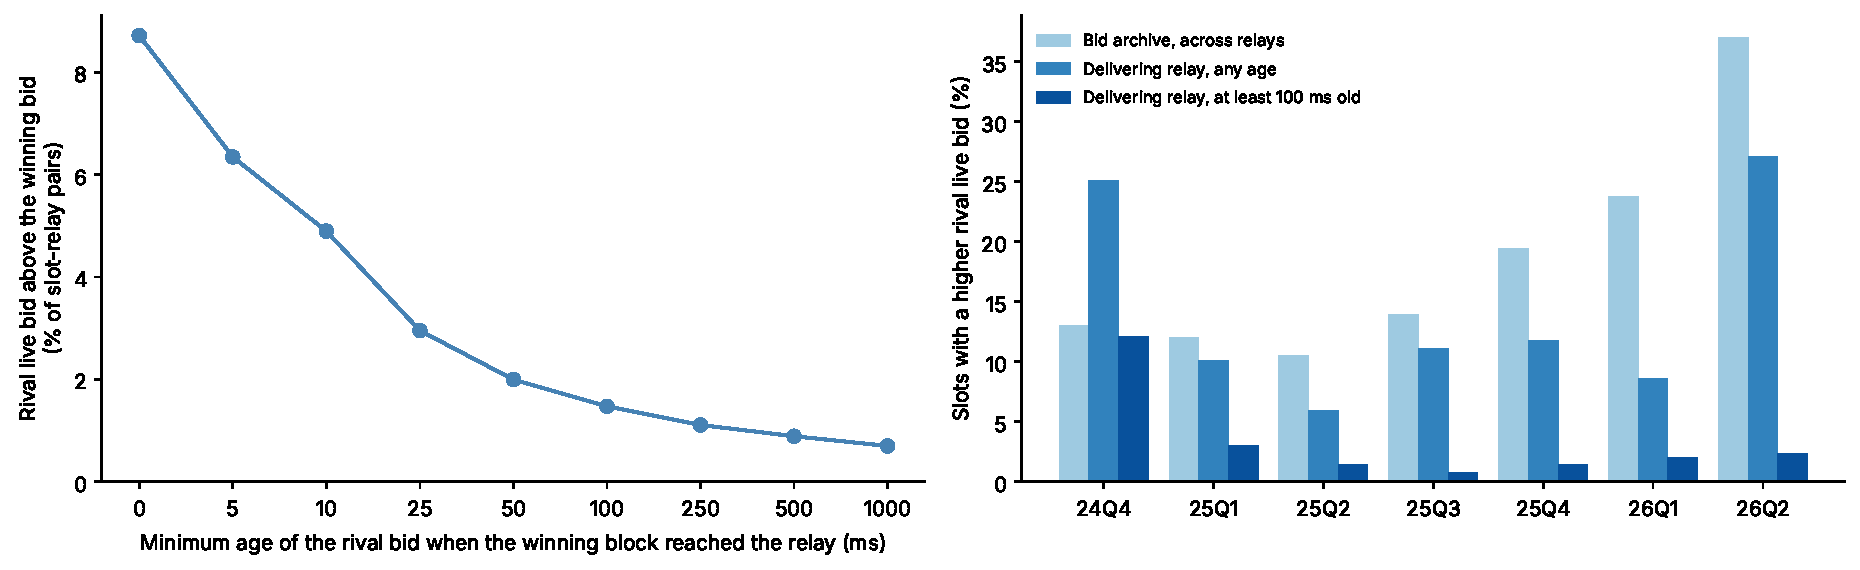
\includegraphics[width=\textwidth]{figures/fig_relay_trace.pdf}
\caption{Same-relay check, 24 sample days. Left: share of slot-relay pairs
in which a rival operator's live bid on the delivering relay exceeds the
winning bid, by minimum age of that bid. Right: share of slots with a higher
rival live bid, by quarter, in the bid archive and on the delivering relay.}
\label{fig:relay_trace}
\end{figure}

\begin{quote}
\textbf{Finding 5a.} \textit{The median slot receives 2,748 bids from 50
builder keys and about 25 operators. When the winning bid arrives it is
1.08\% above the best live bid of any other operator at the median, and no
rival operator is within 1\% in 51\% of slots (re-weighted to market winner
shares; 1.33\% and 55\% in the sample). The margin is 0.33\% when Titan
wins and 3.98\% when beaverbuild does; measured by key it is zero. A
rival's live bid is above the winning bid in 18\% of slots, but on the relay
that delivered the block such bids are a median of 12\,ms old, and one that
is at least 100\,ms old and from one of the five largest operators is
present in 0.55\% of slots.}
\end{quote}

\subsubsection{Block Value}
\label{sec:comp_value}

High-value slots attract more bidders. The median number of operators
bidding is 22, 25 and 27 in the low-, mid- and high-value terciles
($\rho = 0.388$; bootstrap 95\% CI $[0.370, 0.407]$, $B = 1{,}000$), and the
median number of keys 44, 52 and 57 ($\rho = 0.446$). The number of bids is
unrelated to value ($\rho = -0.019$).

More bidders do not translate into a closer contest
(Table~\ref{tab:value}). The tercile medians of the standing margin are
1.22\%, 1.50\% and 1.32\%, the mean number of rivals within 1\% is 0.59,
0.52 and 0.53, and the rank correlation between block value and the standing
margin is slightly positive ($\rho = 0.033$; bootstrap 95\% CI
$[0.011, 0.053]$). Slots with more operators bidding have, if anything,
wider margins ($\rho = 0.153$). The winning bid arrives at nearly the same
time in every tercile (951, 979 and 973\,ms).

\begin{table}[!htbp]
\centering
\caption{The auction by block value tercile}
\label{tab:value}
\begin{tabular}{lrrrrrr}
\toprule
Value & Operators & Keys & Bids & Median & Rival bid & Rivals within \\
tercile & (median) & (median) & (median) & $m_s$ (\%) & higher (\%) & 1\% (mean) \\
\midrule
Low & 22 & 44 & 2{,}687 & 1.219 & 21.2 & 0.59 \\
Mid & 25 & 52 & 3{,}008 & 1.495 & 17.4 & 0.52 \\
High & 27 & 57 & 2{,}542 & 1.324 & 16.9 & 0.53 \\
\bottomrule
\end{tabular}
\end{table}

\begin{quote}
\textbf{Finding 5b.} \textit{More operators bid in high-value slots (median
22, 25 and 27 across value terciles; $\rho = 0.388$), but the winner's
margin over the best rival does not narrow with block value
($\rho = 0.033$) or with the number of operators bidding ($\rho = 0.153$).}
\end{quote}

\subsubsection{Temporal Evolution of the Auction}
\label{sec:comp_evolution}

Table~\ref{tab:quarter} and Figure~\ref{fig:competitiveness_timeseries}
follow the auction through the sample. Participation \emph{declined}. The
median number of operators bidding per slot is 30--31 through the first
quarter of 2025 and 22--23 from the third quarter of 2025; keys per slot
fall from 71 to 43. The number of distinct operators bidding on a median day
falls from 35 in the third quarter of 2024 to 22 in the fourth quarter of
2025, and is 29 at the end of the sample. The decline is not a matter of relay
composition: within Agnostic-delivered slots alone, the average weekly
median is 30.8 operators per slot in both late 2024 and early 2025, and 23.3
and 22.9 from May 2025 and in 2026. Bids per slot move the other way, roughly
doubling between early and mid 2025, so fewer operators are bidding more
often.

\begin{table}[!htbp]
\centering
\small
\caption{The auction by quarter (medians per slot unless stated)}
\label{tab:quarter}
\begin{tabular}{lrrrrrrrr}
\toprule
 & & & & & \multicolumn{2}{c}{Median $m_s$ (\%)} & Rival bid & Operator HHI, \\
Quarter & Slots & Bids & Keys & Operators & Sample & Re-weighted & higher (\%) & all blocks \\
\midrule
2024 Q3 & 9{,}662 & 1{,}979 & 71 & 30 & 1.352 & 2.850 & 22.0 & 4{,}627 \\
2024 Q4 & 56{,}999 & 1{,}516 & 68 & 31 & 0.877 & 3.437 & 14.5 & 4{,}594 \\
2025 Q1 & 291{,}070 & 1{,}942 & 64 & 30 & 2.027 & 2.154 & 12.3 & 3{,}989 \\
2025 Q2 & 196{,}559 & 3{,}355 & 53 & 27 & 2.397 & 2.013 & 10.8 & 3{,}258 \\
2025 Q3 & 155{,}069 & 3{,}994 & 54 & 23 & 1.560 & 0.864 & 13.8 & 3{,}737 \\
2025 Q4 & 151{,}086 & 3{,}040 & 44 & 22 & 1.107 & 0.246 & 21.0 & 3{,}525 \\
2026 Q1 & 187{,}839 & 2{,}608 & 43 & 23 & 0.819 & 0.156 & 25.2 & 3{,}617 \\
2026 Q2 & 171{,}558 & 2{,}950 & 43 & 22 & 0.158 & 0.069 & 35.6 & 3{,}510 \\
\bottomrule
\end{tabular}

\vspace{0.5em}
\footnotesize Re-weighted: to the market's composition of winning operators
in the quarter. The 2024 re-weighted figures rest on fewer than 1,400
beaverbuild-won sample slots and are imprecise. The HHI column is computed
on all MEV-Boost blocks (Table~\ref{tab:market}).
\end{table}

The winner's margin narrowed sharply over the sample. Re-weighted to the
market's winners, the median standing margin is between 2.0\% and 3.4\%
through the second quarter of 2025, 0.86\% in the third, and 0.25\%, 0.16\%
and 0.07\% in the three quarters after. The fall is not only a change in who
wins. When Titan wins, its median margin is 0.6--1.1\% through the second
quarter of 2025 and 0.03--0.09\% in every quarter from the third; when
BuilderNet wins it is 1.4--2.6\% through 2025 and at or below 0.3\% in 2026.
The break coincides with beaverbuild's order flow moving to BuilderNet and
with Quasar's entry (Table~\ref{tab:market}). The share of slots in which a
rival's live bid exceeds the winning bid rises over the same quarters, to
35.6\%; Section~\ref{sec:same_relay} shows that these are bids arriving
within milliseconds of the winner. Margins and near-simultaneous arrivals
tell the same story of a contest that became much tighter from mid-2025.

The margin and the concentration index both fall over the sample, the index
from about 4,600 to 3,500, but week to week they are unrelated: across 88
weeks the rank correlation between the previous week's market operator HHI
and the sample's weekly median margin is $-0.038$ ($p = 0.73$). Eight
quarters are too few to say more than that the two moved together.

\begin{figure}[!htbp]
\centering
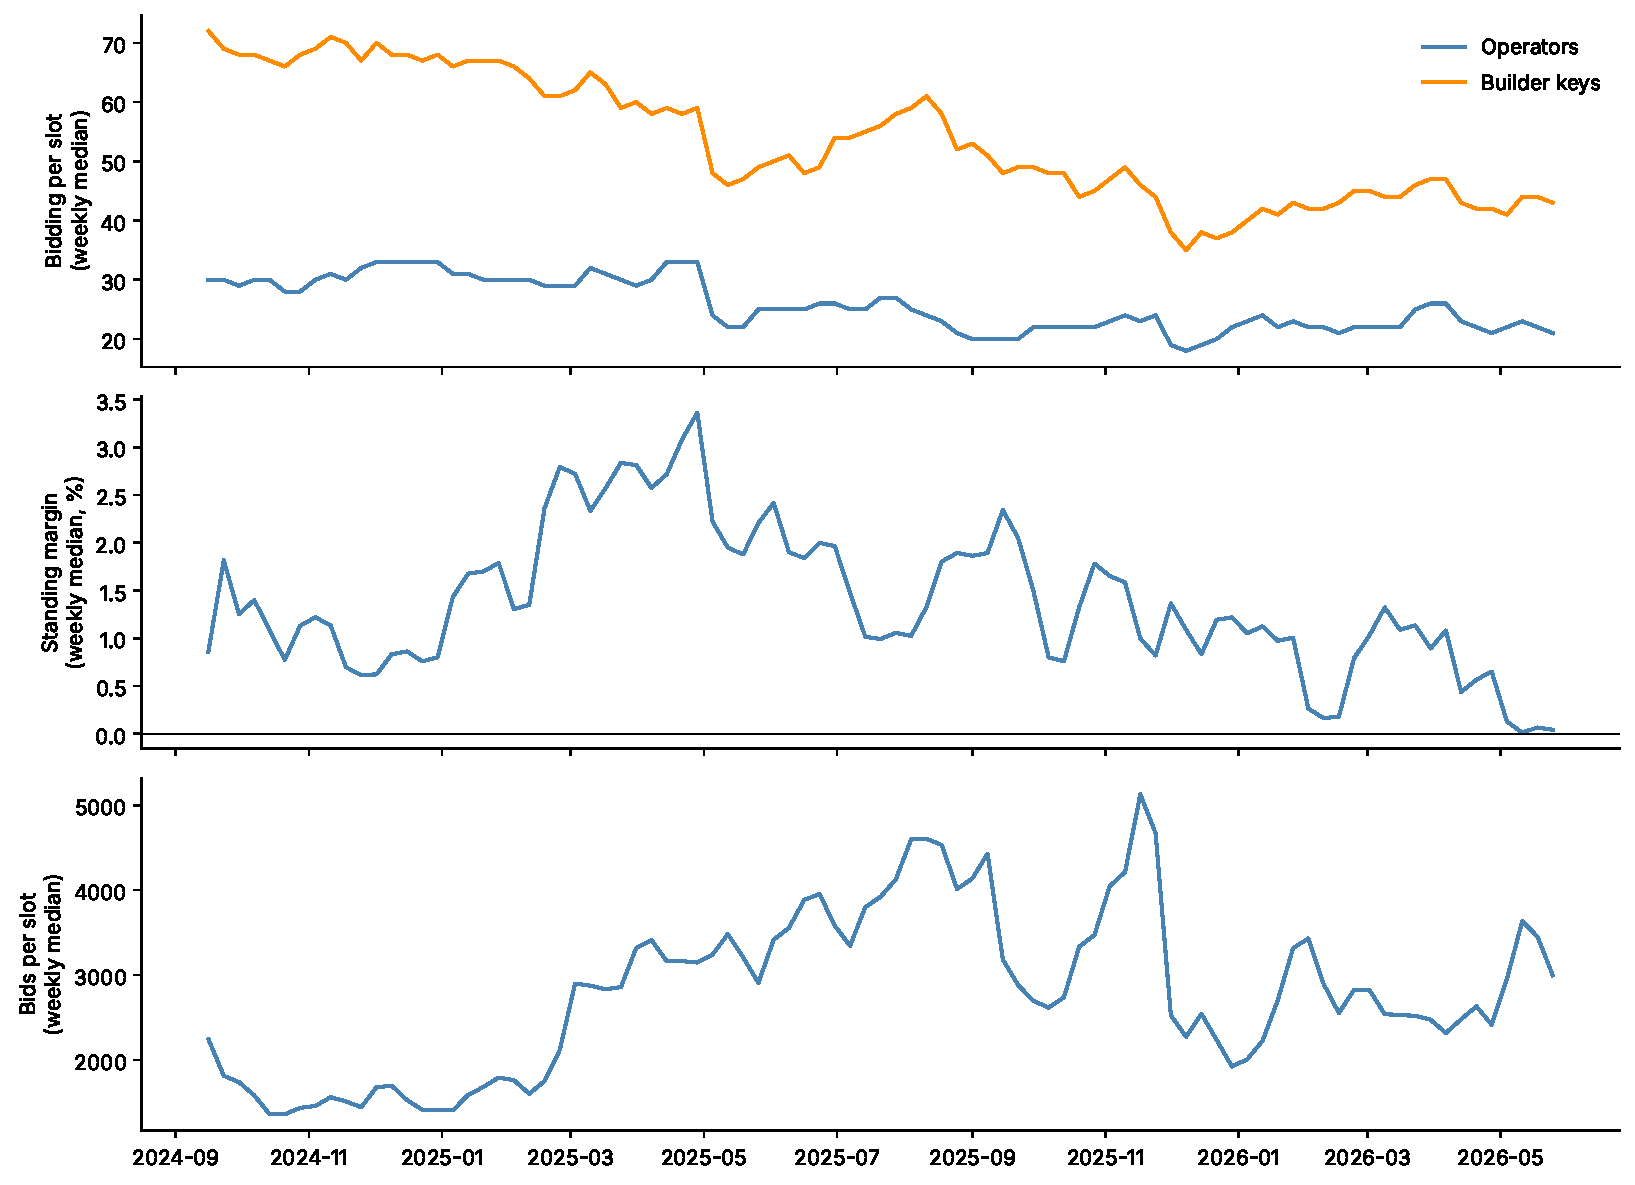
\includegraphics[width=\textwidth]{figures/fig_ab_timeseries.pdf}
\caption{Weekly medians per slot, September 2024 -- May 2026. Top: operators
and builder keys bidding. Middle: standing margin $m_s$. Bottom: bids.}
\label{fig:competitiveness_timeseries}
\end{figure}

\begin{quote}
\textbf{Finding 5c.} \textit{The contest narrowed from mid-2025. Re-weighted
to the market's winners, the median margin over the best rival is 2.0--3.4\%
through the second quarter of 2025 and 0.07--0.25\% from the fourth; when
Titan wins it falls from 0.6--1.1\% to under 0.1\%. Over the same period
fewer operators bid (a median of about 30 per slot falling to 22) while bids
per slot rise, and the concentration index falls from about 4,600 to 3,500.}
\end{quote}

%------------------------------------------------------------------
% SECTION 5.6 — Extended Auction Analysis
%------------------------------------------------------------------
\subsection{Extended Auction Analysis}
\label{sec:extended_auction}

\subsubsection{ETH Price Decomposition}
\label{sec:eth_decomp_sec}

A key limitation of prior PBS analyses is the conflation of ETH price
movements with MEV-specific dynamics. We address this directly using 15,302
hourly ETH/USD price observations from Coinbase (September 2024--May 2026),
matched to delivered payload slots by hour.

Of the 1,219,842 auction-matched slots, 1,218,624 (99.9\%) are matched to
an hourly ETH price observation (only ten hourly bars are missing from the
Coinbase series). We regress log block value (ETH) on log ETH
price and find:

\begin{equation}
\log(v_t) = -4.172 + 0.027 \cdot \log(P_t^{\text{ETH}}) + \varepsilon_t,
\quad R^2 = 0.0001
\label{eq:eth_decomp}
\end{equation}

where $P_t^{\text{ETH}}$ denotes the hourly ETH/USD closing price. ETH price
explains essentially zero variance in block value when both are denominated in
ETH (Spearman $\rho = 0.050$, $p < 10^{-300}$). However, when block value is
converted to USD, the association strengthens substantially (Spearman $\rho =
0.359$, $p < 10^{-300}$), reflecting the mechanical co-movement of any
ETH-denominated quantity with its USD equivalent.

These results establish that the \emph{level} of the ETH price carries no
information about MEV block value in ETH terms. They do not establish that
MEV is unrelated to the ETH market. As reported in
Section~\ref{sec:vol_regimes}, block values rise with ETH price
\emph{volatility}: the hourly median block value has a rank correlation of
0.245 with 24-hour ETH realized volatility, and mean block value is
2.4$\times$ higher in the top ETH-volatility tercile than in the bottom one.
The signed hourly ETH return, by contrast, explains almost nothing (regressing
the hour-to-hour change in log median block value on the hourly ETH return
gives $R^2 = 0.005$). This is the pattern expected if a large share of MEV
comes from arbitrage between centralized and decentralized exchanges, whose
profitability scales with the size of price moves and not their direction
\citep{heimbach2024,wu2025}.

\begin{figure}[!htbp]
\centering
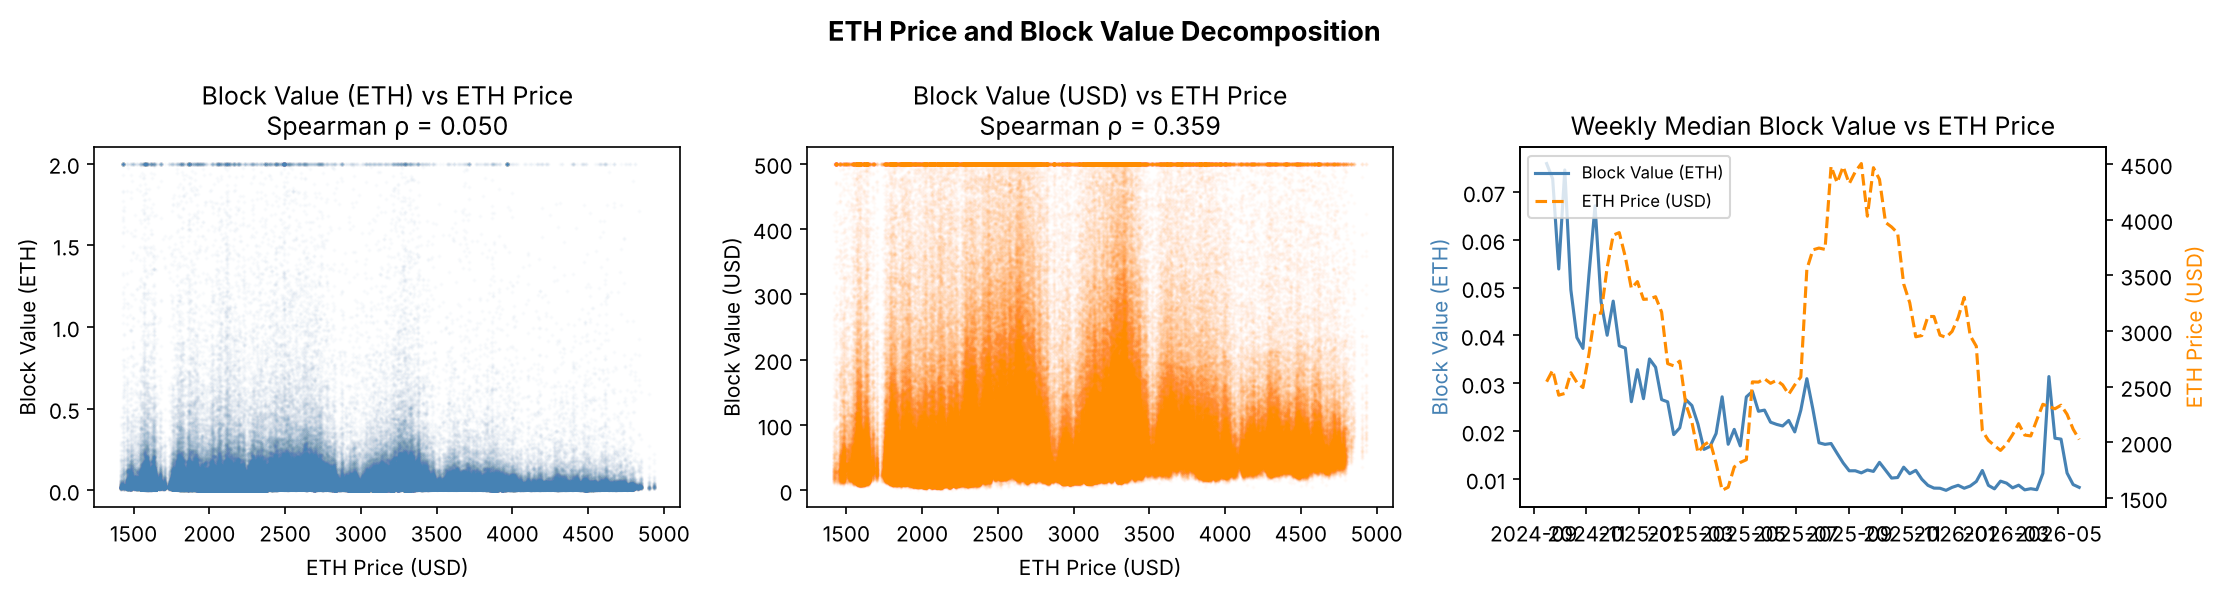
\includegraphics[width=\textwidth]{figures/fig_eth_decomposition.png}
\caption{ETH price and block value decomposition. Left: block value in ETH vs
ETH price (Spearman $\rho = 0.050$); block value in ETH terms is unrelated to
the ETH price level. Centre: block value in USD vs ETH price ($\rho = 0.359$),
reflecting mechanical USD conversion. Right: weekly median block value (ETH,
blue) and ETH price (USD, orange) co-plotted, confirming the visual
decoupling in ETH terms.}
\label{fig:eth_decomp}
\end{figure}

\begin{quote}
\textbf{Finding 6.} \textit{ETH price explains essentially zero variance in
block value when denominated in ETH ($R^2 = 0.0001$, Spearman $\rho = 0.050$),
but explains meaningful variance in USD terms ($\rho = 0.359$). The signed
hourly ETH return also explains almost none ($R^2 = 0.005$). ETH price
\emph{volatility} does co-move with block value ($\rho = 0.245$ at hourly
frequency; mean block value 2.4$\times$ higher in the top ETH-volatility
tercile). MEV in ETH terms responds to the magnitude of price moves, not to
the price level or its direction.}
\end{quote}


\subsubsection{Isolating MEV-Specific Volatility Persistence}
\label{sec:mev_specific}

To check whether the volatility structure documented in Finding~2 could be
produced by signed ETH price movements, we regress the block-value log return
series on the contemporaneous ETH price log return. The regression yields
$R^2 \approx 0.0000$ ($n=1{,}269{,}858$). This test has little power at the
slot level, because the ETH price is observed hourly and its return is
therefore zero for all but one slot per hour; at hourly frequency the signed
ETH return still explains little ($R^2 = 0.005$).

Because the signed ETH return explains essentially none of the variance of
block-value changes, filtering it out leaves the level series, and hence the
GARCH estimates of Finding~2, essentially unchanged. This does not make the
volatility clustering independent of the ETH market: block values rise with
ETH volatility (Finding~6), and ETH volatility is itself persistent. Whether
the persistence in the conditional variance of block values is inherited
from persistence in ETH volatility is not tested here and is left for future
work.

\subsubsection{How Operators Bid}
\label{sec:builder_strat}

Table~\ref{tab:operators} describes the bidding of the five operators with
the most delivered blocks and of three smaller ones discussed below.
Together the five submit 77.4\% of all bids in the sample's slots and win
94.9\% of them.

\begin{table}[!htbp]
\centering
\small
\caption{Bidding by operator, all recorded bids in matched slots}
\label{tab:operators}
\begin{tabular}{lrrrrrrr}
\toprule
 & & Share of & Share of & Wins per & Bid time & After slot & Above winning \\
Operator & Keys & bids (\%) & wins (\%) & 1{,}000 bids & (ms) & start (\%) & value (\%) \\
\midrule
Titan & 29 & 39.3 & 35.4 & 0.30 & 603 & 67.5 & 18.3 \\
BuilderNet & 20 & 17.1 & 23.1 & 0.45 & 175 & 54.7 & 10.2 \\
beaverbuild & 38 & 14.0 & 18.5 & 0.43 & $-$188 & 53.6 & 9.4 \\
Quasar & 11 & 3.4 & 13.6 & 1.33 & $-$503 & 50.7 & 2.8 \\
rsync & 12 & 3.6 & 4.3 & 0.40 & 769 & 76.9 & 6.5 \\
\midrule
BTCS & 12 & 7.1 & 1.6 & 0.07 & $-$1{,}691 & 39.7 & 0.7 \\
Eureka Builder & 163 & 3.2 & 1.0 & 0.11 & $-$1{,}756 & 30.3 & 0.8 \\
bobthebuilder & 25 & 1.5 & 0.9 & 0.19 & 1{,}825 & 96.7 & 40.6 \\
\bottomrule
\end{tabular}

\vspace{0.5em}
\footnotesize Bid time is the bid-weighted mean, over an operator's keys and
days, of the median arrival time of its bids relative to slot start. The
last two columns are the shares of the operator's bids received after slot
start and bid above the delivered value of their slot. Shares are of the sample's
matched slots and differ from the market shares of
Section~\ref{sec:concentration}: Titan wins 47\% of all MEV-Boost blocks and
Quasar 7\%.
\end{table}

The operators differ in how many bids they spend per block won, though the
ratios are those of the sample's slots, in which Titan wins less and Quasar
more than in the market. Titan submits 39\% of all bids. Quasar, which
first bids in April 2025, submits 3.4\%, and wins 1.33 slots per thousand
bids against 0.30--0.45 for the three larger operators; it bids earlier
(half of its bids arrive before slot start) and almost never above the
winning value (2.8\% of its bids, against 9--18\%). A bid above the
delivered value of its slot is a bid the proposer did not take, because it
arrived after the proposer had chosen or was not visible to it, so this
share indicates how much of an operator's bidding falls outside the contest
the proposer saw.

Three smaller operators show how far bidding activity and winning can
diverge. BTCS submits 7.1\% of all bids, twice Quasar's share, mostly well
before slot start, and wins 1.6\% of slots. bobthebuilder bids almost
entirely after slot start (96.7\% of its bids), places 40.6\% of its bids
above the winning value, and wins 0.9\%; a key-level analysis of the same
archive would describe its 25 keys as a cluster of ``late, high-value
bidders'', where grouped they are one operator, a large part of whose
bidding the proposer never acts on. Eureka Builder bids under 163 keys, a
fifth of all keys observed in the sample, of which the median key is active
on a single day: only five of the keys carry its label, and the rest are
attached to it by the blocks they share with those five. It wins 1.0\% of
slots.

\begin{quote}
\textbf{Finding 7.} \textit{Five operators submit 77\% of all bids, with
different bidding intensity: in the sample's slots Titan wins 0.30 blocks
per thousand bids and the most recent entrant, Quasar, 1.33. bobthebuilder bids
almost entirely after slot start, places 41\% of its bids above the winning
value, and wins 0.9\% of slots. Eureka Builder accounts for 163 of the 803
builder keys and 1.0\% of wins.}
\end{quote}

\subsubsection{Bid Timing and Collection Channel in the Bid Archive}
\label{sec:timing_artifact}

Bid timing in the archive's top-bid files differs sharply across relays.
Because these files are small, they are the natural input for timing
studies, and the pattern below would be read as a difference between relays.
Table~\ref{tab:relay_timing} reports the distribution of bid timing by relay,
pooled across all 86.8 million rows of the Q1 2025 top-bid files.

\begin{table}[!htbp]
\centering
\caption{Bid timing (ms relative to slot start) by relay, Q1 2025 top-bid
files ($n = 86{,}805{,}657$)}
\label{tab:relay_timing}
\begin{tabular}{lrrr}
\toprule
Relay & Median (ms) & Mean (ms) & Observations \\
\midrule
Titan & 2{,}497 & 580 & 1{,}512{,}420 \\
BloXroute (regulated) & 2{,}208 & 2{,}421 & 359{,}445 \\
BloXroute (max-profit) & 2{,}104 & 2{,}303 & 237{,}888 \\
Agnostic & 1{,}890 & 1{,}748 & 125{,}789 \\
Flashbots & $-$454 & $-$346 & 790{,}105 \\
Ultrasound & $-$710 & $-$1{,}946 & 83{,}630{,}070 \\
Wenmerge & $-$791 & 1{,}610 & 63 \\
Aestus & $-$4{,}258 & $-$3{,}334 & 126{,}004 \\
Eden Network & $-$4{,}447 & $-$3{,}548 & 15{,}169 \\
SecureRPC & $-$4{,}913 & $-$4{,}225 & 8{,}704 \\
\bottomrule
\end{tabular}
\end{table}

Among relays with more than 10,000 observations, the spread between the
latest-reporting relay (Titan, median $+2{,}497$\,ms) and the
earliest-reporting relay (Eden Network, median $-4{,}447$\,ms) exceeds
6,900\,ms --- more than half a slot duration; including the thinly observed
SecureRPC relay (8,704 observations, median $-4{,}913$\,ms) widens it to
7,410\,ms.

The spread is produced by how the archive collects bids, not by when builders
bid on each relay. The archive's timing field is the time at which the relay
received the bid, relative to slot start, and each bid is stored once, under
the relay through which the collector first saw it, so no bid can be compared
across relays directly. Bids reach the archive through three channels,
recorded in its \texttt{source\_type} field and documented by
\citet{relayscan2024}: Ultrasound's top-bid websocket stream (type~2),
available for that relay only; polling of each relay's data API for the bids
it has received (type~1), at fixed offsets of $-4$, $-2$, $-0.5$, $+0.5$,
$+2$ and $+20$ seconds around slot start; and \texttt{getHeader} polling
(type~0), which carries no bid timestamp and is excluded from all timing
statistics. Table~\ref{tab:source_type} splits the timed Q1 2025 observations
by channel. The stream delivers 83.6 million bids with a median of
$-711$\,ms. Data-API polling delivers 3.2 million with a median of
$+1{,}959$\,ms. Ultrasound's own polled bids have a median of $+2{,}110$\,ms,
in line with the polled bids of BloXroute, Agnostic and Titan ($+1{,}890$ to
$+2{,}497$\,ms). The same relay is `early' or `late' depending only on the
channel.

\begin{table}[!htbp]
\centering
\caption{Bid timing (ms relative to slot start) by collection channel, Q1
2025 top-bid files ($n = 86{,}805{,}657$)}
\label{tab:source_type}
\begin{tabular}{lrr}
\toprule
Channel and relay & Median (ms) & Observations \\
\midrule
Live stream: Ultrasound & $-$711 & 83{,}556{,}614 \\
Data-API polling: Ultrasound & 2{,}110 & 73{,}456 \\
Data-API polling: all other relays & 1{,}948 & 3{,}175{,}587 \\
Data-API polling: all relays & 1{,}959 & 3{,}249{,}043 \\
\bottomrule
\end{tabular}
\end{table}

The mechanism is selection by the top-bid rule. The stream reports every
improvement to Ultrasound's top bid as it happens, so the collector's running
top bid for the slot tracks Ultrasound's in real time. A bid obtained by
polling another relay enters the top-bid file only if it exceeds that running
top bid when it is processed. Bid values rise through the auction, so the
polled bids that qualify are predominantly ones received late, and they are
by construction bids that beat everything the stream had shown. On thinly
used relays (Aestus, Eden Network, SecureRPC) the few qualifying bids are
early ones, recorded before the stream's top bid had risen above them, which
produces their early medians. Relay-level timing differences in the archive
therefore compare all top-bid updates on one relay with the subset of other
relays' bids that overtook them.

\begin{figure}[!htbp]
\centering
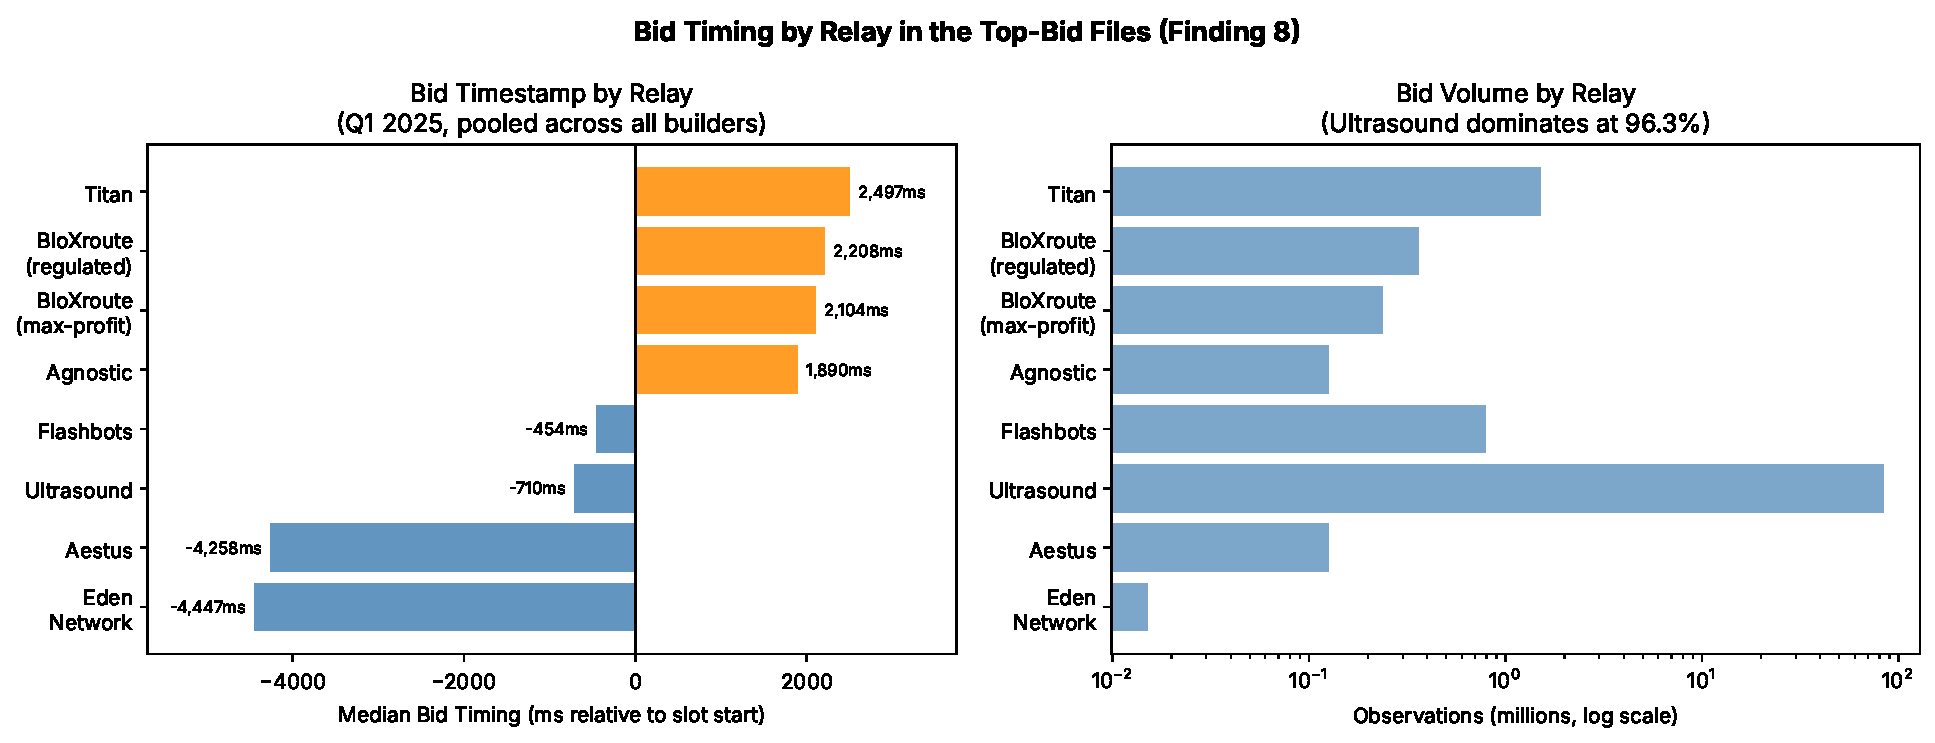
\includegraphics[width=\textwidth]{figures/fig_relay_timing_artifact.pdf}
\caption{Bid timing by relay, Q1 2025 top-bid files
(86.8M observations). Left: median bid timing by relay, pooled across all
builders; positive values indicate bids timestamped after slot start. Right:
bid volume by relay (log scale); Ultrasound, the only relay observed through
a live stream, supplies 96.3\% of all observations
(Table~\ref{tab:source_type}).}
\label{fig:relay_timing}
\end{figure}

\begin{quote}
\textbf{Finding 8.} \textit{Median bid timing in the Relayscan top-bid
files differs by 6,944\,ms between the latest- and earliest-reporting relays with
more than 10,000 observations (Titan vs.\ Eden Network), more than half a
slot. The difference is produced by the collection channel, not by the
relays: bids from Ultrasound's live stream have a median of $-711$\,ms,
while Ultrasound's own data-API-polled bids have a median of $+2{,}110$\,ms,
in line with other relays' polled bids. Bid-timing comparisons in MEV-Boost research
must condition on the collection channel, and relay-level timing differences
in the top-bid files should not be read as differences in builder behaviour.}
\end{quote}

%==================================================================
\section{Discussion}
\label{sec:discussion}
%==================================================================

\subsection{Implications of Persistent Level Volatility}
\label{sec:disc_persistence}

Two results in Section~\ref{sec:garch} deserve comment. The first is
methodological. Block values are non-negative levels, and the common practice
of taking log differences and fitting GARCH---borrowed from asset pricing,
where the object is a price---creates an MA(1) process whose squares carry a
positive lag-one autocorrelation of $(\kappa-1)/(2\kappa+2)$ for an i.i.d.\ level with
kurtosis $\kappa$, with nothing beyond lag one. Ljung-Box tests on such a
series reject at any sample size, and a GARCH fit absorbs the structure into an
inflated ARCH coefficient; under a Student-$t$ likelihood with free degrees of
freedom the inflation is larger still and the constrained fit lands on the
integrated boundary. None of this is evidence about
volatility. The same caution applies to priority fees, bridge flows, and other
level series in blockchain economics.

The second is substantive. On the AR-filtered level, $\hat\alpha \approx 0.04$
and $\hat\beta \approx 0.97$: a shock to the variance of MEV block values decays
slowly, with a half-life well beyond the AR dependence in the level itself.
That persistence sits at the integrated boundary in every specification. For
PBS participants the implication is that elevated-MEV episodes, once begun,
are long-lived relative to the slot clock; for modellers, it is that the
appropriate baseline for MEV block values is an AR--IGARCH-type level model,
or a regime-switching model if the unconditional variance is suspected to
shift across relay regimes, not a return-based model.

\subsection{Concentration by Key and by Operator}
\label{sec:disc_concentration}

The concentration results carry two methodological warnings and a
substantive one. The first warning is that a Herfindahl index computed on
builder public keys measures how operators distribute their bidding across
keys as much as it measures the market. On all MEV-Boost blocks it is lower
than the operator-level index by a factor of nine and never registers even
moderate concentration, in a market where one operator builds half the
blocks. Studies that count builders by key describe a more fragmented
market than the one that exists.
The remedy does not require proprietary data: public labels cover 99.9\% of
blocks, and where labels are missing, keys that submit the same block can
be joined with no false merges in our sample. Exact ties in bid value, by
contrast, joined keys of different builders and should not be used as
evidence of common control.

The second is that an index computed on the delivered payloads of some
relays is an index of the builders who use those relays. Our own five-relay
sample, which covers 31\% of MEV-Boost blocks, put Titan at 35\% of blocks
when it built 47\%, showed its share halving while it rose, and gave an HHI
a quarter below the market's. Concentration should be measured on
all relays, and results from relay subsets should be read as statements
about those relays.

The substantive result is that block building is a highly concentrated
market by the conventional threshold in every week of the sample, with one
operator building 47\% of blocks and five building 97\%. It is less
concentrated than it was: the index falls by about a quarter between late
2024 and 2026. BuilderNet was launched to address this concentration
\citep{buildernet2024}, but the label is not what lowered the index: an
index that treats beaverbuild and BuilderNet as one operator falls by the
same amount, because the combined share of the two halves. What lowered it
is that the order flow beaverbuild's builder won did not all arrive at
BuilderNet, and that Quasar, which did not exist at the start of the
sample, builds a sixth of blocks at the end. The leading positions other
than Titan's are therefore contestable, consistent with a market in which
the binding advantage is access to order flow that can move between
operators \citep{wu2025,oz2024}, while Titan's share has only grown. Whether
blocks built on shared infrastructure by several organisations should count
as one competitor is a question an HHI cannot settle, and it bears directly
on censorship-resistance analysis.

\subsection{What the Bids Show About Competition}
\label{sec:disc_efficiency}

The auction findings in Section~\ref{sec:auction} can be summarised as a
contest that was often one-sided through mid-2025 and has been close since.
Thousands of bids arrive in a slot from around 25 operators. Over the whole
sample, re-weighted to the market's winners, the best live rival bid is
1.08\% below the winning bid at the median when it lands, and in half of
slots no rival is within 1\%. But that average joins two regimes. Through
the second quarter of 2025 the median margin is 2--3\%; from the fourth it
is 0.1--0.3\%, and when Titan wins, which is half the time, it is a few
hundredths of a percent.

The size of the margin depends on getting the operators right. It is zero
by key, 0.74\% when keys are grouped by shared blocks alone, 1.33\% with
public labels, and 1.49\% if the BuilderNet partners are one operator (all
in the sample). Every improvement in the grouping moves it the same way,
because the error is always the same: a sibling key mistaken for a rival.
It also depends on whose auctions are sampled: Titan wins by a third of a
percent and beaverbuild by four, so a sample that under-represents Titan
overstates the margin.

The slots in which a rival's bid appears higher than the winner's turn out
to be evidence of how tight the contest is in time, not of proposers
forgoing value. On the relay that delivered the block, the higher rival bid
had typically arrived 12\,ms before the winning block; bids that were higher
and at least 100\,ms old are present in 2.4\% of slots and come mostly from
builders whose bids proposers apparently could not take. That
near-simultaneous arrivals become more frequent exactly as margins collapse
suggests that competition among the leading operators is now expressed in
latency as much as in price.

Margins do not respond to the cross-sectional variables one would expect.
They do not narrow in high-value slots, although more operators bid there,
and they are not smaller in slots with more operators. What moved them was
a change in who competes: the margin collapses in the quarter in which
beaverbuild's flow moves to BuilderNet and Quasar begins to win, and stays
low.

The decline in participation (from about 30 to 22 operators per slot)
accompanies this. Fewer operators bid at the end of the sample than at the
start, those that remain bid more often, and the contest among them is
closer. This is consistent with a market in which the fixed costs of
competitive block building (orderflow access, latency infrastructure)
select for a small set of capable operators who then compete hard with one
another. For proposers the implication is favourable: with margins near
zero, the winning builder is bidding close to what its best rival bids.

\subsection{Limitations}
\label{sec:limitations}

The baseline volatility measure is constructed from block values themselves,
on a window that contains the current block; Section~\ref{sec:vol_regimes}
reports how the results change on a non-overlapping window and with ETH
price volatility as an external measure. The ETH price series is hourly, so
the ETH-volatility comparison is made at hourly frequency only. The GARCH persistence estimate on the
level sits at the integrated boundary, which is also the signature of
unconditional-variance shifts in a sample with a change in relay composition;
regime-switching or structural-break specifications would distinguish the two.

BloXroute contributed approximately 66\% of the deduplicated sample
(Agnostic 22\%, Ultra Sound 8\%, Flashbots 5\%, Aestus $<$1\%), and its
records begin in the week of 6 January 2025; late 2024 is observed through
Agnostic alone. The sample is therefore not representative of the market,
and Section~\ref{sec:concentration} measures how unrepresentative: it holds
31\% of MEV-Boost blocks, under-represents Titan by a quarter over the whole
period and by more than half in some quarters, and over-represents Quasar
and BuilderNet. The concentration results do not use it. Everything else
does. The block-value results (Sections~\ref{sec:vol_regimes}
to~\ref{sec:temporal} and the ETH-price decomposition) describe the sequence
of blocks delivered through these relays, and the change in relay
composition in January 2025 is a candidate source of the variance shifts
discussed in Section~\ref{sec:garch}. The auction results are re-weighted to
the market's composition of winners by quarter, which corrects for who wins
but not for any other way in which slots delivered through these relays
differ from the rest, for example in the proposers who use them. The 2024
quarters have too few sample slots won by beaverbuild, which then built
half of all blocks, for the re-weighted figures of those quarters to be
precise.

Bid-level data from relay APIs was unavailable for direct collection due to
authentication restrictions. The auction analysis in Section~\ref{sec:auction}
instead uses the Relayscan.io Bid Archive \citep{relayscan2024}, and inherits
its coverage. The archive holds the bids its collector observed, through one
live stream and periodic polling of the other relays
(Section~\ref{sec:timing_artifact}); bids that were replaced between polls on
a polled relay may be missing, and the winning block is not found among the
recorded bids in 2.1\% of slots. Timestamps are those reported by each
relay, and rows obtained by \texttt{getHeader} polling carry none. The
collection channels are as documented by \citet{relayscan2024}; we did not
re-implement the collector. The archive does not record when the proposer
requested a header or which relays it queried, and it stores a bid once
however many relays received it. The standing margin therefore rests on two
assumptions stated in Section~\ref{sec:method}: that the proposer chose at
about the time the winning bid arrived, and that a key's most recent bid is
its live bid on every relay. Section~\ref{sec:same_relay} tests them on a
sample, but that sample is 24 days, its per-relay source polls relay APIs
and so may miss bids, it has no Ultra Sound bids after April 2025, and it
contains the winning block in only a fifth of slots on Titan Relay; the
2.4\% and 0.55\% figures are established on the relays it does cover, chiefly
BloXroute and Agnostic. Margins are computed from each slot's 40 highest-bidding keys
at or below the winning value, reduced to the eight best rival groups, and
the per-slot operator count uses within-day shared-block links only.

Operators rest on public labels, which we did not construct. The labels
come from a mapping of keys to builder names and from the
\texttt{extra\_data} field of delivered blocks \citep{dataalways2024}; both
are self-reported by builders, and a builder can set \texttt{extra\_data}
to anything. They agree with each other for 218 of the 220 keys that have
both, and with shared-block behaviour for every labelled key, which is the
best check available without private information. Labels cover 229 of 803
keys; the remaining 574 keys, which submit 4.7\% of bids and win 0.3\% of
slots, are grouped by shared blocks or left as single-key operators, and
keys of one operator that never share a block remain separate. Labels also
do not settle what an operator is. BuilderNet is one label run by several
organisations, and beaverbuild is a separate label for part of the sample
and part of BuilderNet for the rest; we report concentration and margins
both ways and do not claim that either is the correct unit for every
question.

%==================================================================
\section{Conclusion}
\label{sec:conclusion}
%==================================================================

This paper characterises MEV block values as a stochastic process across
multiple market regimes, using 1,271,079 delivered payload observations from five
MEV-Boost relays spanning September 2024 through May 2026, supplemented by
the 3.7 billion bids recorded for 1,219,842 of those slots in the
Relayscan.io Bid Archive and by the delivered payloads of all relays. Eight findings emerge, all estimated on the full
20-month sample:

\begin{enumerate}
\item \textbf{Volatility regime sensitivity:} Block values rise with recent
block-value volatility ($\rho = 0.494$, $H = 266{,}905$, $p < 10^{-300}$;
$\rho = 0.414$ on a non-overlapping earlier window). The median block is
2.3--2.7$\times$ larger in the high-volatility tercile; the ratio of means is
7.0$\times$ on the baseline window and 3.5$\times$ on the non-overlapping
one. Block values also rise with ETH price volatility ($\rho = 0.245$ at
hourly frequency).

\item \textbf{Persistent level volatility:} Block values are a level process;
differencing them induces spurious ARCH. On the AR-filtered level, MEV block
values exhibit highly persistent conditional heteroskedasticity
($\hat\alpha = 0.044$, $\hat\beta = 0.965$, $\hat\alpha + \hat\beta = 1.01$),
stable across filter orders and near-integrated in both sample halves
(persistence 1.002 and 1.075).

\item \textbf{High concentration by operator:} Builders bid under many keys.
On all 4.1 million MEV-Boost blocks, grouping keys by public label and
shared blocks raises the HHI from 344 to 3,080 (3,883 with beaverbuild
counted as part of BuilderNet); Titan builds 47\% of blocks, five operators
97\%, and the weekly operator HHI exceeds 2,500 in every week, while falling
from about 4,600 to 3,500 over the sample. Shared blocks identify operators
without a false merge; exact value ties do not. A five-relay sample
mis-states builder shares by up to forty percentage points.

\item \textbf{Robust temporal seasonality:} Both intraday ($H = 65{,}875$) and
day-of-week ($H = 33{,}590$) patterns are highly significant across the full
20-month period. Median block values peak during 13:00--17:00 UTC and are
highest on Mondays.

\item \textbf{An auction that became close:} The median slot receives 2,748
bids from 50 keys and about 25 operators. Re-weighted to the market's
winners, the winning bid is 1.08\% above the best live bid of any other
operator at the median (zero by key), but the margin falls from 2--3\%
through mid-2025 to 0.1--0.3\% from late 2025, and to a few hundredths of
a percent when Titan wins. A rival's bid appears higher in 18\% of slots; on
the delivering relay such bids are a median of 12\,ms old, and one at least
100\,ms old from a leading operator is present in 0.55\% of slots. More
operators bid in high-value slots ($\rho = 0.388$) but the margin does not
narrow with value.

\item \textbf{MEV tracks ETH volatility, not the ETH price level:} The ETH
price level explains essentially zero variance in block value in ETH terms
($R^2 = 0.0001$, $\rho = 0.050$), and the signed hourly return almost none,
but block values rise with ETH price volatility ($\rho = 0.245$ at hourly
frequency).

\item \textbf{Operators bid differently:} Five operators submit 77\% of bids;
in the sample's slots, wins per thousand bids range from 0.30 for Titan to
1.33 for Quasar, the most recent entrant. bobthebuilder bids almost
entirely after slot start and places 41\% of its bids above the winning
value; Eureka Builder accounts for 163 of the 803 keys and 1.0\% of wins.

\item \textbf{Timing in the top-bid files reflects the collection channel:}
Median bid timing differs by more than six seconds across relays in the
archive's top-bid files because of how bids are collected (live stream
versus polling), not because of the relays. Those files also continue past
the winning bid in 96\% of slots and contain the winning block in 29\%.
\end{enumerate}

Future work should repeat the auction analysis on a slot sample drawn from
all relays, which the bid archive permits; extend the same-relay check from
24 days to the full sample and to the relays it does not cover; measure, with proposer-side
data, the latency race among the leading operators that the near-simultaneous
bids point to; test whether the persistence in block-value volatility is
inherited from persistence in ETH price volatility, using intra-hour price
data; apply
regime-switching models to the level series to separate long-memory volatility
from unconditional-variance shifts; and pursue authenticated relay access across a
broader, market-share-weighted relay set to assess the sensitivity of the
reported findings to the BloXroute-dominated composition of the current sample.

%==================================================================

\bibliographystyle{plainnat}
\begin{thebibliography}{99}

\bibitem[Lamoureux and Lastrapes, 1990]{lamoureux1990}
Lamoureux, C. G. and Lastrapes, W. D. (1990).
Persistence in variance, structural change, and the GARCH model.
\textit{Journal of Business \& Economic Statistics}, 8(2):225--234.

\bibitem[Bahrani et al., 2024]{bahrani2024}
Bahrani, M., Garimidi, P., and Roughgarden, T. (2024).
Centralization in block building and proposer-builder separation.
\textit{Financial Cryptography and Data Security (FC 2024)}; arXiv:2401.12120.

\bibitem[Bollerslev, 1986]{bollerslev1986}
Bollerslev, T. (1986).
Generalized autoregressive conditional heteroskedasticity.
\textit{Journal of Econometrics}, 31(3):307--327.

\bibitem[Bollerslev and Wooldridge, 1992]{bollerslevwooldridge1992}
Bollerslev, T. and Wooldridge, J. M. (1992).
Quasi-maximum likelihood estimation and inference in dynamic models with time-varying covariances.
\textit{Econometric Reviews}, 11(2):143--172.

\bibitem[BuilderNet, 2025]{beaverbuild2025}
BuilderNet (2025).
Beaverbuild $\rightarrow$ BuilderNet.
\url{https://buildernet.org/blog/beaverbuild}

\bibitem[Buterin, 2021]{buterin2021}
Buterin, V. (2021).
Two-slot proposer/builder separation.
\textit{Ethereum Research Forum}.
\url{https://ethresear.ch/t/two-slot-proposer-builder-separation/10980}

\bibitem[Daian et al., 2020]{daian2020}
Daian, P., Goldfeder, S., Kell, T., Li, Y., Zhao, X., Bentov, I.,
Breidenbach, L., and Juels, A. (2020).
Flash boys 2.0: Frontrunning in decentralized exchanges, miner extractable
value, and consensus instability.
\textit{IEEE Symposium on Security and Privacy}.

\bibitem[Data Always, 2024]{dataalways2024}
Data Always (2024).
mevboost-data: MEV-Boost winning bid data.
\url{https://github.com/dataalways/mevboost-data}

\bibitem[Engle, 1982]{engle1982}
Engle, R. F. (1982).
Autoregressive conditional heteroscedasticity with estimates of the variance
of United Kingdom inflation.
\textit{Econometrica}, 50(4):987--1007.

\bibitem[Engle and Bollerslev, 1986]{engle_bollerslev1986}
Engle, R. F. and Bollerslev, T. (1986).
Modelling the persistence of conditional variances.
\textit{Econometric Reviews}, 5(1):1--50.

\bibitem[ethPandaOps, 2024]{xatu2024}
ethPandaOps (2024).
Xatu data: MEV relay bid traces.
\url{https://ethpandaops.io/data/xatu/}

\bibitem[Flashbots, 2022]{flashbots2022}
Flashbots (2022).
MEV-Boost: Proposer-builder separation for Ethereum validators.
\textit{Flashbots Documentation}.
\url{https://docs.flashbots.net/flashbots-mev-boost/introduction}

\bibitem[Flashbots, 2024]{buildernet2024}
Flashbots (2024).
Introducing BuilderNet.
\url{https://buildernet.org/blog/introducing-buildernet}

\bibitem[Heimbach et al., 2024]{heimbach2024}
Heimbach, L., Pahari, V., and Schertenleib, E. (2024).
Non-atomic arbitrage in decentralized finance.
\textit{IEEE Symposium on Security and Privacy (SP)}, pages 3866--3884.

\bibitem[Hirschman, 1945]{hirschman1945}
Hirschman, A. O. (1945).
\textit{National Power and the Structure of Foreign Trade}.
University of California Press.

\bibitem[\"Oz et al., 2024]{oz2024}
\"Oz, B., Sui, D., Thiery, T., and Matthes, F. (2024).
Who wins Ethereum block building auctions and why?
\textit{Advances in Financial Technologies (AFT 2024)}; arXiv:2407.13931.

\bibitem[Qin et al., 2022]{qin2022}
Qin, K., Zhou, L., and Gervais, A. (2022).
Quantifying blockchain extractable value: How dark is the forest?
\textit{IEEE Symposium on Security and Privacy}.

\bibitem[Relayscan, 2024]{relayscan2024}
Flashbots (2024).
Relayscan.io Bid Archive.
\textit{Flashbots Open Data}.
\url{https://bidarchive.relayscan.io}

\bibitem[Wang et al., 2024]{wang2024}
Wang, S., Huang, Y., Zhang, W., Huang, Y., Wang, X., and Tang, J. (2024).
Private order flows and builder bidding dynamics: The road to monopoly in
Ethereum's block building market.
\textit{arXiv preprint arXiv:2410.12352}.

\bibitem[Wahrst\"atter et al., 2023]{wahrstatter2023}
Wahrst\"atter, A., Ernstberger, J., Yaish, A., Zhou, L., Qin, K.,
Tsuchiya, T., Steinhorst, S., Svetinovic, D., Christin, N., Wattenhofer, R.,
and Gervais, A. (2023).
Blockchain censorship.
\textit{Proceedings of the ACM Web Conference}.

\bibitem[Wu et al., 2023]{wu2023}
Wu, F., Thiery, T., Leonardos, S., and Ventre, C. (2023).
Strategic bidding wars in on-chain auctions.
\textit{arXiv preprint arXiv:2312.14510}.

\bibitem[Wu et al., 2024]{wu2024}
Wu, F., Thiery, T., Leonardos, S., and Ventre, C. (2024).
From competition to centralization: The oligopoly in Ethereum block building
auctions.
\textit{arXiv preprint arXiv:2412.18074}.

\bibitem[Wu et al., 2025]{wu2025}
Wu, F., Sui, D., Thiery, T., and Pai, M. (2025).
Measuring CEX-DEX extracted value and searcher profitability: The darkest of
the MEV dark forest.
\textit{arXiv preprint arXiv:2507.13023}.

\end{thebibliography}

\end{document}
